\section{Travessia em árvores binárias de busca}

\begin{frame}[fragile]{Definição}
	\begin{itemize}
		\item A {travessia de uma árvore} é o processo de visitar cada 
		nó {exatamente uma} vez

        \item Visitar significa processar, de algum modo, o nó visitado

		\item A travessia pode ser interpretada como o processo de 
		{linearização} de uma árvore

		\item A definição de travessia {não} especifica a {ordem} 
		na qual os nós devem ser visitados

		\item O número de travessias possíveis de uma árvore é igual o número 
		de {permutações} de seus nós 

		\item Se a árvore tem $n$ nós, terá $n!$ travessias distintas

		\item Há, contudo, dois tipos {especiais} de travessia: 
		travessia por {extensão} e travessia por {profundidade}
	\end{itemize} 

\end{frame}
 
\begin{frame}[fragile]{Travessia por extensão e por profundidade}

	\begin{itemize}
		\item {A travessia por {extensão} consiste em visitar cada nó 
		começando do nível mais {baixo} (ou mais alto) e seguindo para 
		{baixo} (ou para cima) nível a nível, visitando {todos} 
		os nós {daquele} nível da esquerda para a direita (ou em sentido 
		oposto)}

        \item Dada a natureza da travessia por extensão, sua implementação pode requerer 
            o auxílio de uma fila

        \item {A travessia por {profundidade} consiste em ir o mais longe 
        possível à {esquerda}, retornar até o primeiro cruzamento, tomar à 
        {direita} e novamente ir o máximo para a {esquerda}, até que 
        todos os nós tenham sido visitados} 

        \item A travessia por profundidade pode ser implementada recursivamente

        \item Também pode ser implementada iterativamente, com o auxílio de uma pilha
	\end{itemize}

\end{frame}

\begin{frame}[fragile]{Travessias por profundidade notáveis}

	\begin{itemize}
		\item A definição de travessia por profundidade {não} especifica o {momento} em que o 
		nó deve ser visitado

		\item Há 3 {tarefas} de interesse neste caso:

		\begin{enumerate}
			\item {Visitar} o nó (\code{c}{V})

			\item Realizar a travessia da subárvore da {esquerda} (\code{c}{L})

			\item Realizar a travessia da subárvore da {direita} (\code{c}{R})

		\end{enumerate}

		\item As 6 possíveis {permutações} destas tarefas são travessias 
		por profundidade {válidas}

	    \item As travessias por profundidade mais comuns são:

        \begin{enumerate}
            \item pré-ordem: \code{c}{VLR}

            \item em-ordem: \code{c}{LVR}

            \item pós-ordem: \code{c}{LRV}
        \end{enumerate}

    \end{itemize}
\end{frame}

\begin{frame}[fragile]{Exemplo de inserção em árvore binária de busca}

    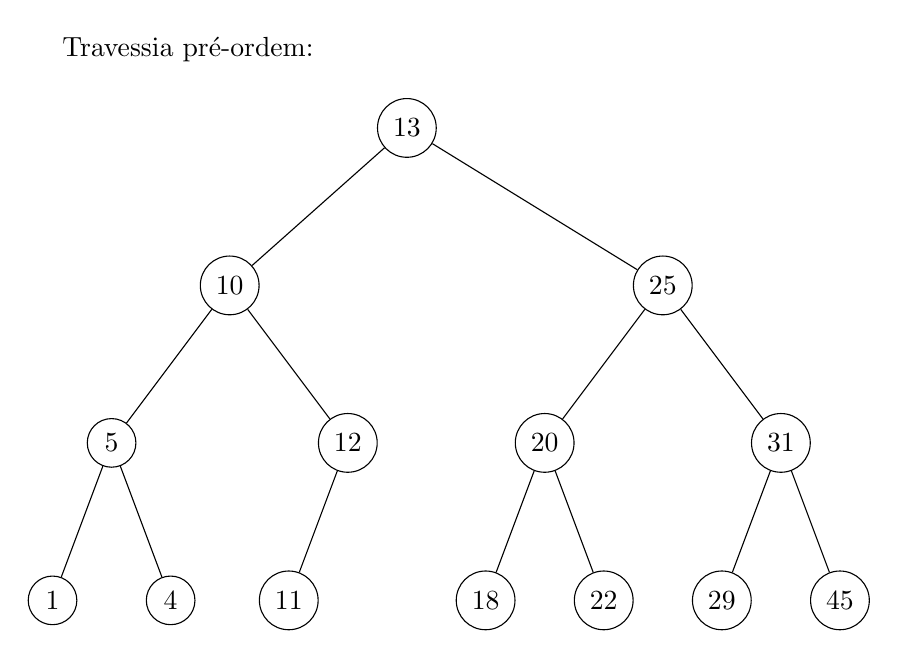
\begin{tikzpicture}

        \begin{scope}
            \node[anchor=west] (X) at (0, 6) { Travessia pré-ordem: };

            \node[circle,draw] (A) at (4.5, 5) { $13$ };
            \node[circle,draw] (B) at (2.25, 3) { $10$ };
            \node[circle,draw] (C) at (7.75, 3) { $25$ };
            \node[circle,draw] (D) at (0.75, 1) { $5$ };
            \node[circle,draw] (E) at (3.75, 1) { $12$ };
            \node[circle,draw] (F) at (6.25, 1) { $20$ };
            \node[circle,draw] (G) at (9.25, 1) { $31$ };
            \node[circle,draw] (H) at (0, -1) { $1$ };
            \node[circle,draw] (I) at (1.5, -1) { $4$ };
            \node[circle,draw] (J) at (3, -1) { $11$ };
            \node[circle,draw] (L) at (5.5, -1) { $18$ };
            \node[circle,draw] (M) at (7, -1) { $22$ };
            \node[circle,draw] (N) at (8.5, -1) { $29$ };
            \node[circle,draw] (O) at (10, -1) { $45$ };

            \draw (A) -- (B);
            \draw (A) -- (C);
            \draw (B) -- (D);
            \draw (B) -- (E);
            \draw (C) -- (F);
            \draw (C) -- (G);

            \draw (D) -- (H);
            \draw (D) -- (I);
            \draw (E) -- (J);
            \draw (F) -- (L);
            \draw (F) -- (M);
            \draw (G) -- (N);
            \draw (G) -- (O);
        \end{scope}
    \end{tikzpicture}

\end{frame}

\begin{frame}[fragile]{Exemplo de inserção em árvore binária de busca}

    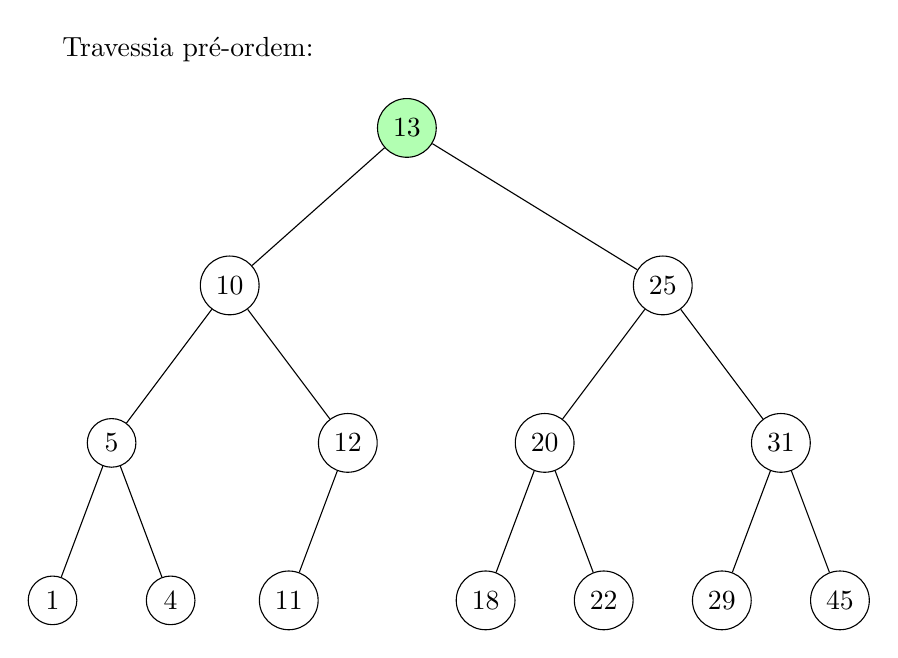
\begin{tikzpicture}

        \begin{scope}
            \node[anchor=west] (X) at (0, 6) { Travessia pré-ordem: };

            \node[circle,draw,fill=green!30] (A) at (4.5, 5) { $13$ };
            \node[circle,draw] (B) at (2.25, 3) { $10$ };
            \node[circle,draw] (C) at (7.75, 3) { $25$ };
            \node[circle,draw] (D) at (0.75, 1) { $5$ };
            \node[circle,draw] (E) at (3.75, 1) { $12$ };
            \node[circle,draw] (F) at (6.25, 1) { $20$ };
            \node[circle,draw] (G) at (9.25, 1) { $31$ };
            \node[circle,draw] (H) at (0, -1) { $1$ };
            \node[circle,draw] (I) at (1.5, -1) { $4$ };
            \node[circle,draw] (J) at (3, -1) { $11$ };
            \node[circle,draw] (L) at (5.5, -1) { $18$ };
            \node[circle,draw] (M) at (7, -1) { $22$ };
            \node[circle,draw] (N) at (8.5, -1) { $29$ };
            \node[circle,draw] (O) at (10, -1) { $45$ };

            \draw (A) -- (B);
            \draw (A) -- (C);
            \draw (B) -- (D);
            \draw (B) -- (E);
            \draw (C) -- (F);
            \draw (C) -- (G);

            \draw (D) -- (H);
            \draw (D) -- (I);
            \draw (E) -- (J);
            \draw (F) -- (L);
            \draw (F) -- (M);
            \draw (G) -- (N);
            \draw (G) -- (O);
        \end{scope}
    \end{tikzpicture}

\end{frame}

\begin{frame}[fragile]{Exemplo de inserção em árvore binária de busca}

    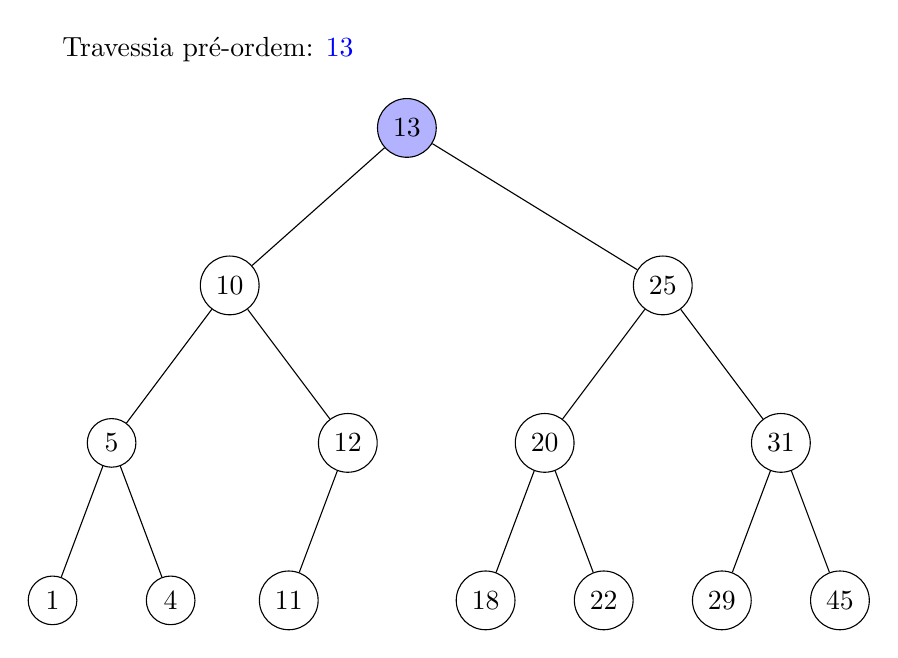
\begin{tikzpicture}

        \begin{scope}
            \node[anchor=west] (X) at (0, 6) { Travessia pré-ordem: \textcolor{blue}{13} };

            \node[circle,draw,fill=blue!30] (A) at (4.5, 5) { $13$ };
            \node[circle,draw] (B) at (2.25, 3) { $10$ };
            \node[circle,draw] (C) at (7.75, 3) { $25$ };
            \node[circle,draw] (D) at (0.75, 1) { $5$ };
            \node[circle,draw] (E) at (3.75, 1) { $12$ };
            \node[circle,draw] (F) at (6.25, 1) { $20$ };
            \node[circle,draw] (G) at (9.25, 1) { $31$ };
            \node[circle,draw] (H) at (0, -1) { $1$ };
            \node[circle,draw] (I) at (1.5, -1) { $4$ };
            \node[circle,draw] (J) at (3, -1) { $11$ };
            \node[circle,draw] (L) at (5.5, -1) { $18$ };
            \node[circle,draw] (M) at (7, -1) { $22$ };
            \node[circle,draw] (N) at (8.5, -1) { $29$ };
            \node[circle,draw] (O) at (10, -1) { $45$ };

            \draw (A) -- (B);
            \draw (A) -- (C);
            \draw (B) -- (D);
            \draw (B) -- (E);
            \draw (C) -- (F);
            \draw (C) -- (G);

            \draw (D) -- (H);
            \draw (D) -- (I);
            \draw (E) -- (J);
            \draw (F) -- (L);
            \draw (F) -- (M);
            \draw (G) -- (N);
            \draw (G) -- (O);
        \end{scope}
    \end{tikzpicture}

\end{frame}


\begin{frame}[fragile]{Exemplo de inserção em árvore binária de busca}

    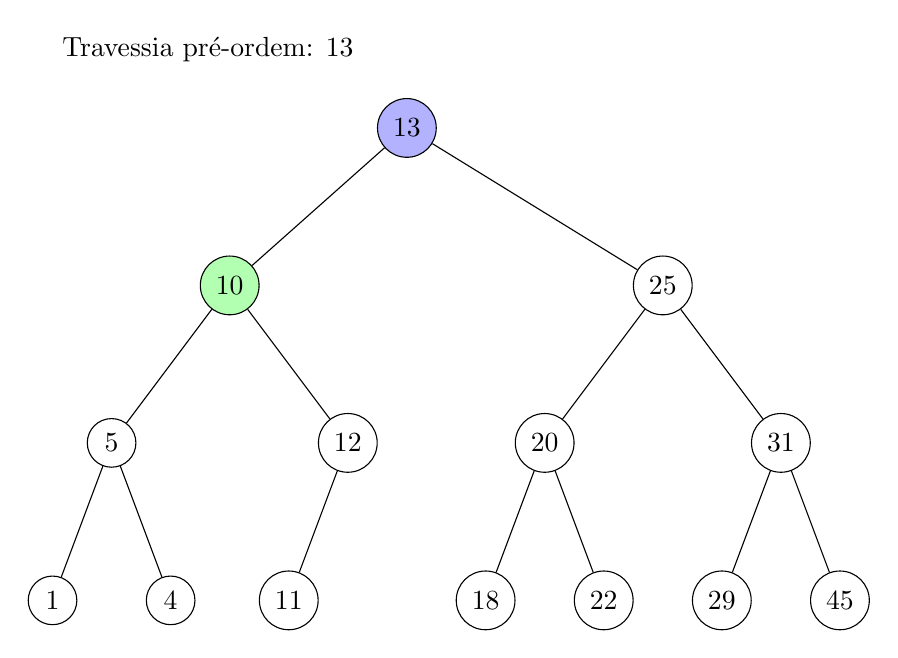
\begin{tikzpicture}

        \begin{scope}
            \node[anchor=west] (X) at (0, 6) { Travessia pré-ordem: 13 \textcolor{blue}{} };

            \node[circle,draw,fill=blue!30] (A) at (4.5, 5) { $13$ };
            \node[circle,draw,fill=green!30] (B) at (2.25, 3) { $10$ };
            \node[circle,draw] (C) at (7.75, 3) { $25$ };
            \node[circle,draw] (D) at (0.75, 1) { $5$ };
            \node[circle,draw] (E) at (3.75, 1) { $12$ };
            \node[circle,draw] (F) at (6.25, 1) { $20$ };
            \node[circle,draw] (G) at (9.25, 1) { $31$ };
            \node[circle,draw] (H) at (0, -1) { $1$ };
            \node[circle,draw] (I) at (1.5, -1) { $4$ };
            \node[circle,draw] (J) at (3, -1) { $11$ };
            \node[circle,draw] (L) at (5.5, -1) { $18$ };
            \node[circle,draw] (M) at (7, -1) { $22$ };
            \node[circle,draw] (N) at (8.5, -1) { $29$ };
            \node[circle,draw] (O) at (10, -1) { $45$ };

            \draw (A) -- (B);
            \draw (A) -- (C);
            \draw (B) -- (D);
            \draw (B) -- (E);
            \draw (C) -- (F);
            \draw (C) -- (G);

            \draw (D) -- (H);
            \draw (D) -- (I);
            \draw (E) -- (J);
            \draw (F) -- (L);
            \draw (F) -- (M);
            \draw (G) -- (N);
            \draw (G) -- (O);
        \end{scope}
    \end{tikzpicture}

\end{frame}

\begin{frame}[fragile]{Exemplo de inserção em árvore binária de busca}

    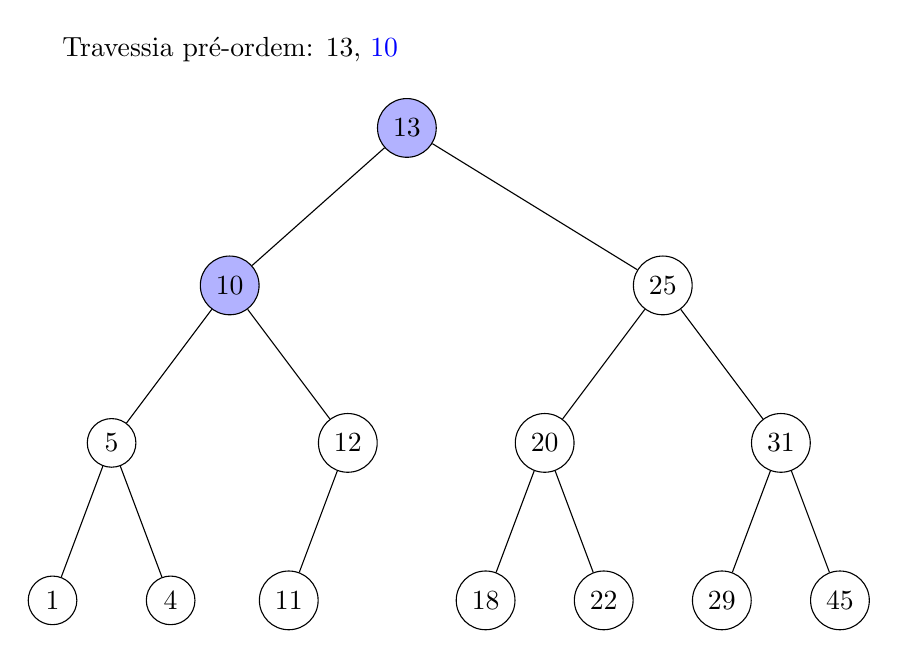
\begin{tikzpicture}

        \begin{scope}
            \node[anchor=west] (X) at (0, 6) { Travessia pré-ordem: 13, \textcolor{blue}{10} };

            \node[circle,draw,fill=blue!30] (A) at (4.5, 5) { $13$ };
            \node[circle,draw,fill=blue!30] (B) at (2.25, 3) { $10$ };
            \node[circle,draw] (C) at (7.75, 3) { $25$ };
            \node[circle,draw] (D) at (0.75, 1) { $5$ };
            \node[circle,draw] (E) at (3.75, 1) { $12$ };
            \node[circle,draw] (F) at (6.25, 1) { $20$ };
            \node[circle,draw] (G) at (9.25, 1) { $31$ };
            \node[circle,draw] (H) at (0, -1) { $1$ };
            \node[circle,draw] (I) at (1.5, -1) { $4$ };
            \node[circle,draw] (J) at (3, -1) { $11$ };
            \node[circle,draw] (L) at (5.5, -1) { $18$ };
            \node[circle,draw] (M) at (7, -1) { $22$ };
            \node[circle,draw] (N) at (8.5, -1) { $29$ };
            \node[circle,draw] (O) at (10, -1) { $45$ };

            \draw (A) -- (B);
            \draw (A) -- (C);
            \draw (B) -- (D);
            \draw (B) -- (E);
            \draw (C) -- (F);
            \draw (C) -- (G);

            \draw (D) -- (H);
            \draw (D) -- (I);
            \draw (E) -- (J);
            \draw (F) -- (L);
            \draw (F) -- (M);
            \draw (G) -- (N);
            \draw (G) -- (O);
        \end{scope}
    \end{tikzpicture}

\end{frame}

\begin{frame}[fragile]{Exemplo de inserção em árvore binária de busca}

    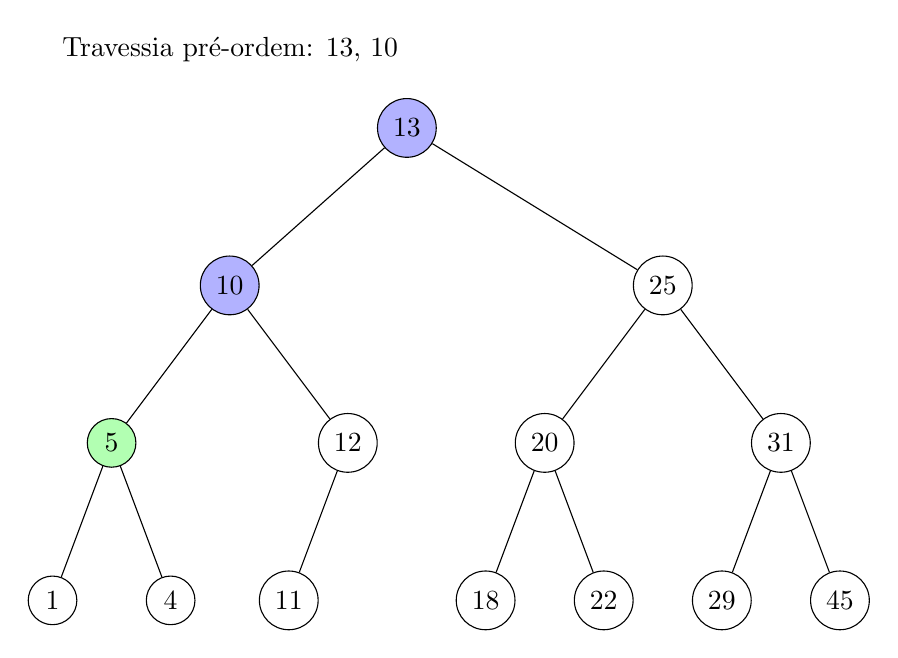
\begin{tikzpicture}

        \begin{scope}
            \node[anchor=west] (X) at (0, 6) { Travessia pré-ordem: 13, 10 \textcolor{blue}{} };

            \node[circle,draw,fill=blue!30] (A) at (4.5, 5) { $13$ };
            \node[circle,draw,fill=blue!30] (B) at (2.25, 3) { $10$ };
            \node[circle,draw] (C) at (7.75, 3) { $25$ };
            \node[circle,draw,fill=green!30] (D) at (0.75, 1) { $5$ };
            \node[circle,draw] (E) at (3.75, 1) { $12$ };
            \node[circle,draw] (F) at (6.25, 1) { $20$ };
            \node[circle,draw] (G) at (9.25, 1) { $31$ };
            \node[circle,draw] (H) at (0, -1) { $1$ };
            \node[circle,draw] (I) at (1.5, -1) { $4$ };
            \node[circle,draw] (J) at (3, -1) { $11$ };
            \node[circle,draw] (L) at (5.5, -1) { $18$ };
            \node[circle,draw] (M) at (7, -1) { $22$ };
            \node[circle,draw] (N) at (8.5, -1) { $29$ };
            \node[circle,draw] (O) at (10, -1) { $45$ };

            \draw (A) -- (B);
            \draw (A) -- (C);
            \draw (B) -- (D);
            \draw (B) -- (E);
            \draw (C) -- (F);
            \draw (C) -- (G);

            \draw (D) -- (H);
            \draw (D) -- (I);
            \draw (E) -- (J);
            \draw (F) -- (L);
            \draw (F) -- (M);
            \draw (G) -- (N);
            \draw (G) -- (O);
        \end{scope}
    \end{tikzpicture}

\end{frame}

\begin{frame}[fragile]{Exemplo de inserção em árvore binária de busca}

    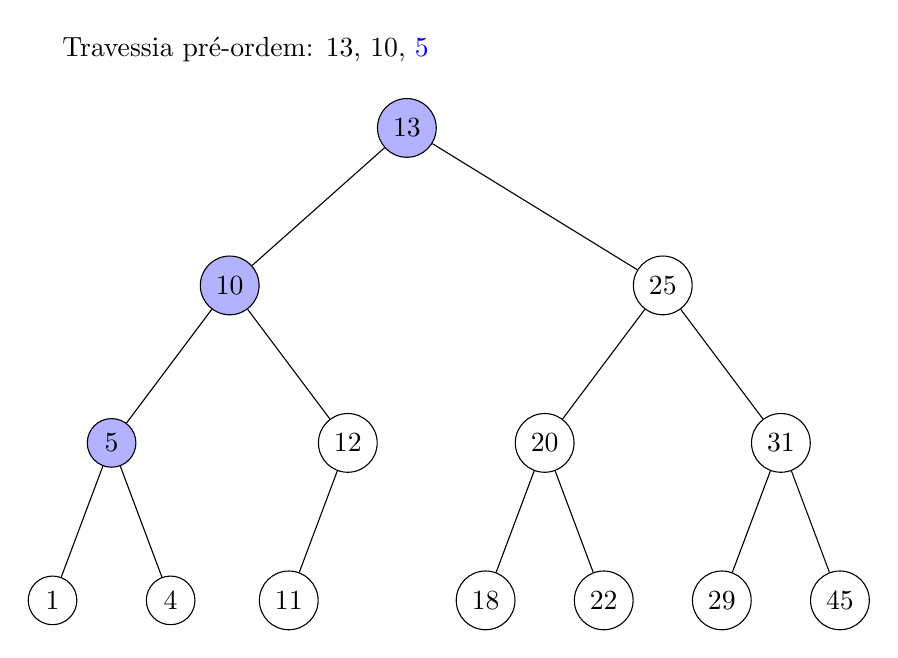
\begin{tikzpicture}

        \begin{scope}
            \node[anchor=west] (X) at (0, 6) { Travessia pré-ordem: 13, 10, \textcolor{blue}{5} };

            \node[circle,draw,fill=blue!30] (A) at (4.5, 5) { $13$ };
            \node[circle,draw,fill=blue!30] (B) at (2.25, 3) { $10$ };
            \node[circle,draw] (C) at (7.75, 3) { $25$ };
            \node[circle,draw,fill=blue!30] (D) at (0.75, 1) { $5$ };
            \node[circle,draw] (E) at (3.75, 1) { $12$ };
            \node[circle,draw] (F) at (6.25, 1) { $20$ };
            \node[circle,draw] (G) at (9.25, 1) { $31$ };
            \node[circle,draw] (H) at (0, -1) { $1$ };
            \node[circle,draw] (I) at (1.5, -1) { $4$ };
            \node[circle,draw] (J) at (3, -1) { $11$ };
            \node[circle,draw] (L) at (5.5, -1) { $18$ };
            \node[circle,draw] (M) at (7, -1) { $22$ };
            \node[circle,draw] (N) at (8.5, -1) { $29$ };
            \node[circle,draw] (O) at (10, -1) { $45$ };

            \draw (A) -- (B);
            \draw (A) -- (C);
            \draw (B) -- (D);
            \draw (B) -- (E);
            \draw (C) -- (F);
            \draw (C) -- (G);

            \draw (D) -- (H);
            \draw (D) -- (I);
            \draw (E) -- (J);
            \draw (F) -- (L);
            \draw (F) -- (M);
            \draw (G) -- (N);
            \draw (G) -- (O);
        \end{scope}
    \end{tikzpicture}

\end{frame}

\begin{frame}[fragile]{Exemplo de inserção em árvore binária de busca}

    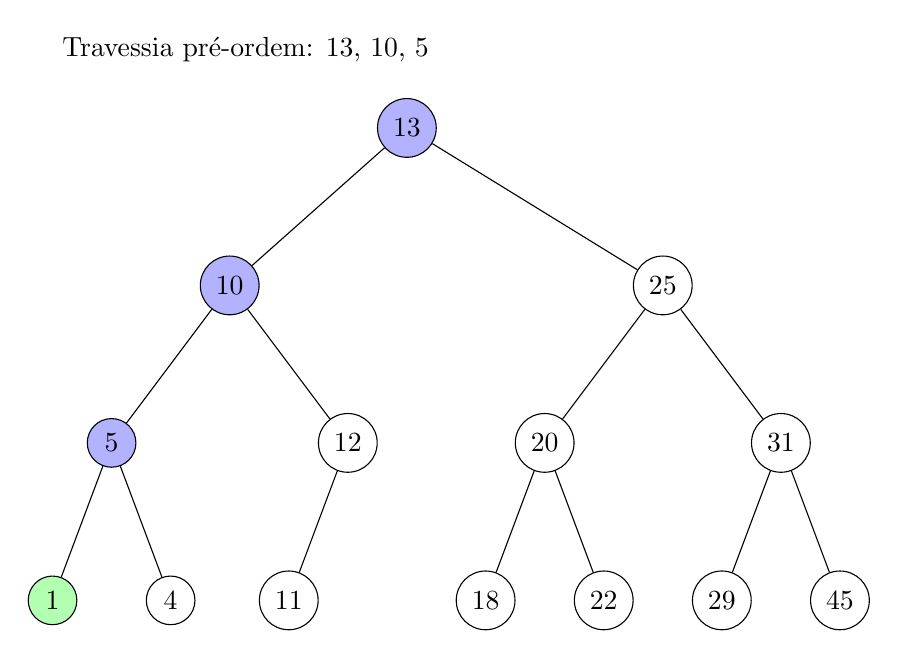
\begin{tikzpicture}

        \begin{scope}
            \node[anchor=west] (X) at (0, 6) { Travessia pré-ordem: 13, 10, 5\textcolor{blue}{} };

            \node[circle,draw,fill=blue!30] (A) at (4.5, 5) { $13$ };
            \node[circle,draw,fill=blue!30] (B) at (2.25, 3) { $10$ };
            \node[circle,draw] (C) at (7.75, 3) { $25$ };
            \node[circle,draw,fill=blue!30] (D) at (0.75, 1) { $5$ };
            \node[circle,draw] (E) at (3.75, 1) { $12$ };
            \node[circle,draw] (F) at (6.25, 1) { $20$ };
            \node[circle,draw] (G) at (9.25, 1) { $31$ };
            \node[circle,draw,fill=green!30] (H) at (0, -1) { $1$ };
            \node[circle,draw] (I) at (1.5, -1) { $4$ };
            \node[circle,draw] (J) at (3, -1) { $11$ };
            \node[circle,draw] (L) at (5.5, -1) { $18$ };
            \node[circle,draw] (M) at (7, -1) { $22$ };
            \node[circle,draw] (N) at (8.5, -1) { $29$ };
            \node[circle,draw] (O) at (10, -1) { $45$ };

            \draw (A) -- (B);
            \draw (A) -- (C);
            \draw (B) -- (D);
            \draw (B) -- (E);
            \draw (C) -- (F);
            \draw (C) -- (G);

            \draw (D) -- (H);
            \draw (D) -- (I);
            \draw (E) -- (J);
            \draw (F) -- (L);
            \draw (F) -- (M);
            \draw (G) -- (N);
            \draw (G) -- (O);
        \end{scope}
    \end{tikzpicture}

\end{frame}

\begin{frame}[fragile]{Exemplo de inserção em árvore binária de busca}

    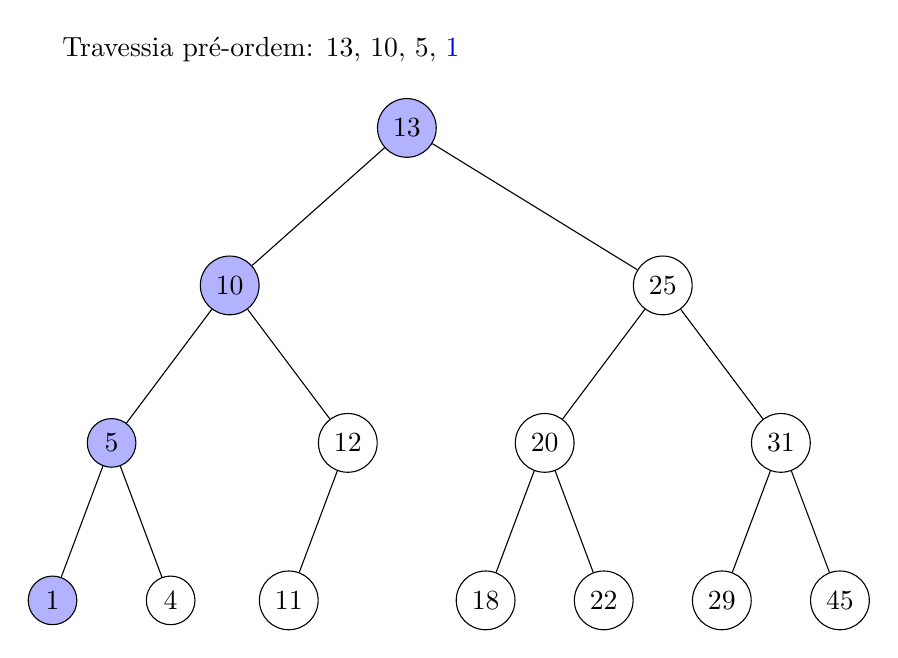
\begin{tikzpicture}

        \begin{scope}
            \node[anchor=west] (X) at (0, 6) { Travessia pré-ordem: 13, 10, 5, \textcolor{blue}{1} };

            \node[circle,draw,fill=blue!30] (A) at (4.5, 5) { $13$ };
            \node[circle,draw,fill=blue!30] (B) at (2.25, 3) { $10$ };
            \node[circle,draw] (C) at (7.75, 3) { $25$ };
            \node[circle,draw,fill=blue!30] (D) at (0.75, 1) { $5$ };
            \node[circle,draw] (E) at (3.75, 1) { $12$ };
            \node[circle,draw] (F) at (6.25, 1) { $20$ };
            \node[circle,draw] (G) at (9.25, 1) { $31$ };
            \node[circle,draw,fill=blue!30] (H) at (0, -1) { $1$ };
            \node[circle,draw] (I) at (1.5, -1) { $4$ };
            \node[circle,draw] (J) at (3, -1) { $11$ };
            \node[circle,draw] (L) at (5.5, -1) { $18$ };
            \node[circle,draw] (M) at (7, -1) { $22$ };
            \node[circle,draw] (N) at (8.5, -1) { $29$ };
            \node[circle,draw] (O) at (10, -1) { $45$ };

            \draw (A) -- (B);
            \draw (A) -- (C);
            \draw (B) -- (D);
            \draw (B) -- (E);
            \draw (C) -- (F);
            \draw (C) -- (G);

            \draw (D) -- (H);
            \draw (D) -- (I);
            \draw (E) -- (J);
            \draw (F) -- (L);
            \draw (F) -- (M);
            \draw (G) -- (N);
            \draw (G) -- (O);
        \end{scope}
    \end{tikzpicture}

\end{frame}

\begin{frame}[fragile]{Exemplo de inserção em árvore binária de busca}

    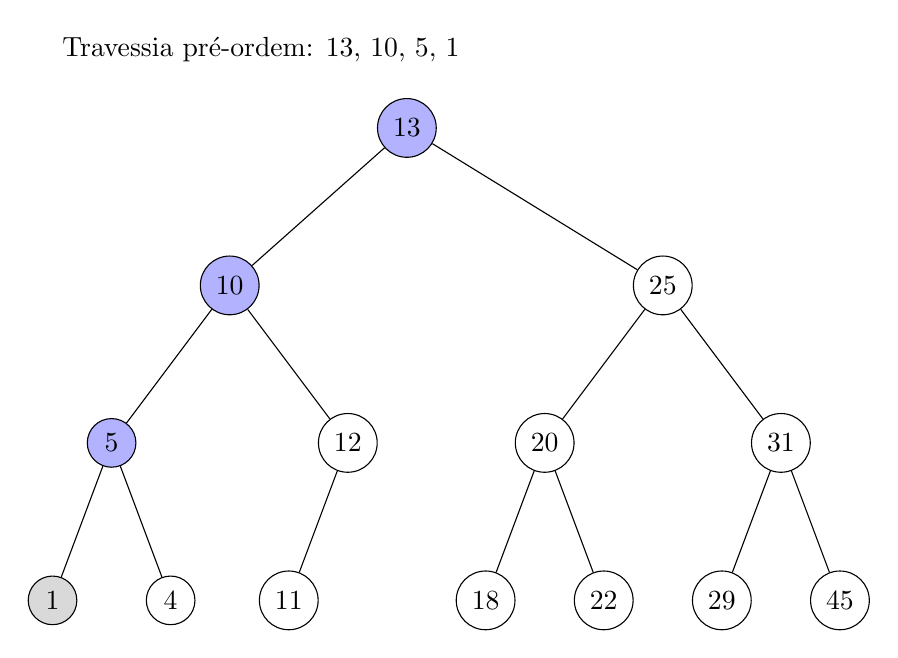
\begin{tikzpicture}

        \begin{scope}
            \node[anchor=west] (X) at (0, 6) { Travessia pré-ordem: 13, 10, 5, 1\textcolor{blue}{} };

            \node[circle,draw,fill=blue!30] (A) at (4.5, 5) { $13$ };
            \node[circle,draw,fill=blue!30] (B) at (2.25, 3) { $10$ };
            \node[circle,draw] (C) at (7.75, 3) { $25$ };
            \node[circle,draw,fill=blue!30] (D) at (0.75, 1) { $5$ };
            \node[circle,draw] (E) at (3.75, 1) { $12$ };
            \node[circle,draw] (F) at (6.25, 1) { $20$ };
            \node[circle,draw] (G) at (9.25, 1) { $31$ };
            \node[circle,draw,fill=gray!30] (H) at (0, -1) { $1$ };
            \node[circle,draw] (I) at (1.5, -1) { $4$ };
            \node[circle,draw] (J) at (3, -1) { $11$ };
            \node[circle,draw] (L) at (5.5, -1) { $18$ };
            \node[circle,draw] (M) at (7, -1) { $22$ };
            \node[circle,draw] (N) at (8.5, -1) { $29$ };
            \node[circle,draw] (O) at (10, -1) { $45$ };

            \draw (A) -- (B);
            \draw (A) -- (C);
            \draw (B) -- (D);
            \draw (B) -- (E);
            \draw (C) -- (F);
            \draw (C) -- (G);

            \draw (D) -- (H);
            \draw (D) -- (I);
            \draw (E) -- (J);
            \draw (F) -- (L);
            \draw (F) -- (M);
            \draw (G) -- (N);
            \draw (G) -- (O);
        \end{scope}
    \end{tikzpicture}

\end{frame}

\begin{frame}[fragile]{Exemplo de inserção em árvore binária de busca}

    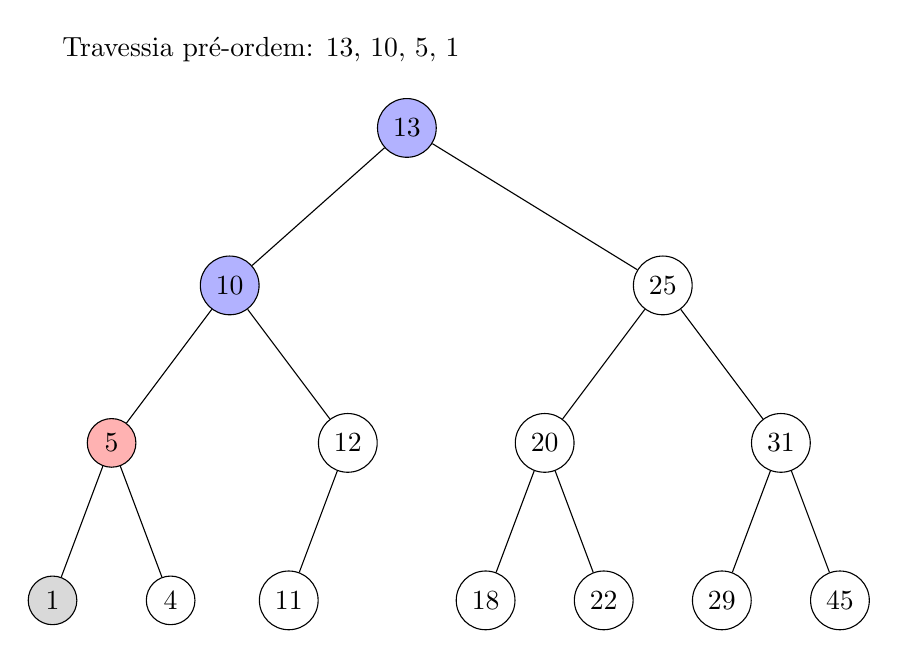
\begin{tikzpicture}

        \begin{scope}
            \node[anchor=west] (X) at (0, 6) { Travessia pré-ordem: 13, 10, 5, 1\textcolor{blue}{} };

            \node[circle,draw,fill=blue!30] (A) at (4.5, 5) { $13$ };
            \node[circle,draw,fill=blue!30] (B) at (2.25, 3) { $10$ };
            \node[circle,draw] (C) at (7.75, 3) { $25$ };
            \node[circle,draw,fill=red!30] (D) at (0.75, 1) { $5$ };
            \node[circle,draw] (E) at (3.75, 1) { $12$ };
            \node[circle,draw] (F) at (6.25, 1) { $20$ };
            \node[circle,draw] (G) at (9.25, 1) { $31$ };
            \node[circle,draw,fill=gray!30] (H) at (0, -1) { $1$ };
            \node[circle,draw] (I) at (1.5, -1) { $4$ };
            \node[circle,draw] (J) at (3, -1) { $11$ };
            \node[circle,draw] (L) at (5.5, -1) { $18$ };
            \node[circle,draw] (M) at (7, -1) { $22$ };
            \node[circle,draw] (N) at (8.5, -1) { $29$ };
            \node[circle,draw] (O) at (10, -1) { $45$ };

            \draw (A) -- (B);
            \draw (A) -- (C);
            \draw (B) -- (D);
            \draw (B) -- (E);
            \draw (C) -- (F);
            \draw (C) -- (G);

            \draw (D) -- (H);
            \draw (D) -- (I);
            \draw (E) -- (J);
            \draw (F) -- (L);
            \draw (F) -- (M);
            \draw (G) -- (N);
            \draw (G) -- (O);
        \end{scope}
    \end{tikzpicture}

\end{frame}

\begin{frame}[fragile]{Exemplo de inserção em árvore binária de busca}

    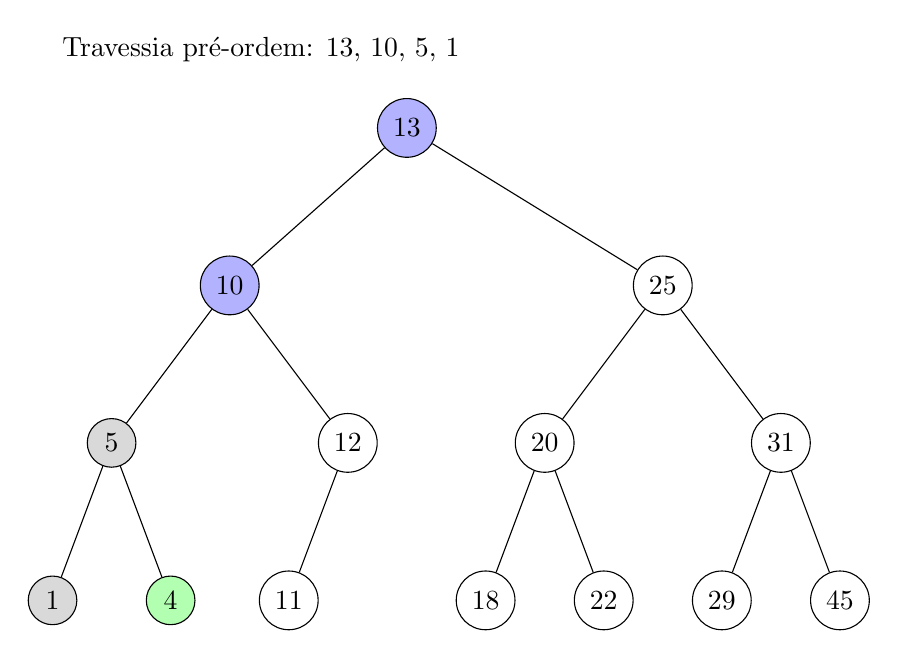
\begin{tikzpicture}

        \begin{scope}
            \node[anchor=west] (X) at (0, 6) { Travessia pré-ordem: 13, 10, 5, 1\textcolor{blue}{} };

            \node[circle,draw,fill=blue!30] (A) at (4.5, 5) { $13$ };
            \node[circle,draw,fill=blue!30] (B) at (2.25, 3) { $10$ };
            \node[circle,draw] (C) at (7.75, 3) { $25$ };
            \node[circle,draw,fill=gray!30] (D) at (0.75, 1) { $5$ };
            \node[circle,draw] (E) at (3.75, 1) { $12$ };
            \node[circle,draw] (F) at (6.25, 1) { $20$ };
            \node[circle,draw] (G) at (9.25, 1) { $31$ };
            \node[circle,draw,fill=gray!30] (H) at (0, -1) { $1$ };
            \node[circle,draw,fill=green!30] (I) at (1.5, -1) { $4$ };
            \node[circle,draw] (J) at (3, -1) { $11$ };
            \node[circle,draw] (L) at (5.5, -1) { $18$ };
            \node[circle,draw] (M) at (7, -1) { $22$ };
            \node[circle,draw] (N) at (8.5, -1) { $29$ };
            \node[circle,draw] (O) at (10, -1) { $45$ };

            \draw (A) -- (B);
            \draw (A) -- (C);
            \draw (B) -- (D);
            \draw (B) -- (E);
            \draw (C) -- (F);
            \draw (C) -- (G);

            \draw (D) -- (H);
            \draw (D) -- (I);
            \draw (E) -- (J);
            \draw (F) -- (L);
            \draw (F) -- (M);
            \draw (G) -- (N);
            \draw (G) -- (O);
        \end{scope}
    \end{tikzpicture}

\end{frame}

\begin{frame}[fragile]{Exemplo de inserção em árvore binária de busca}

    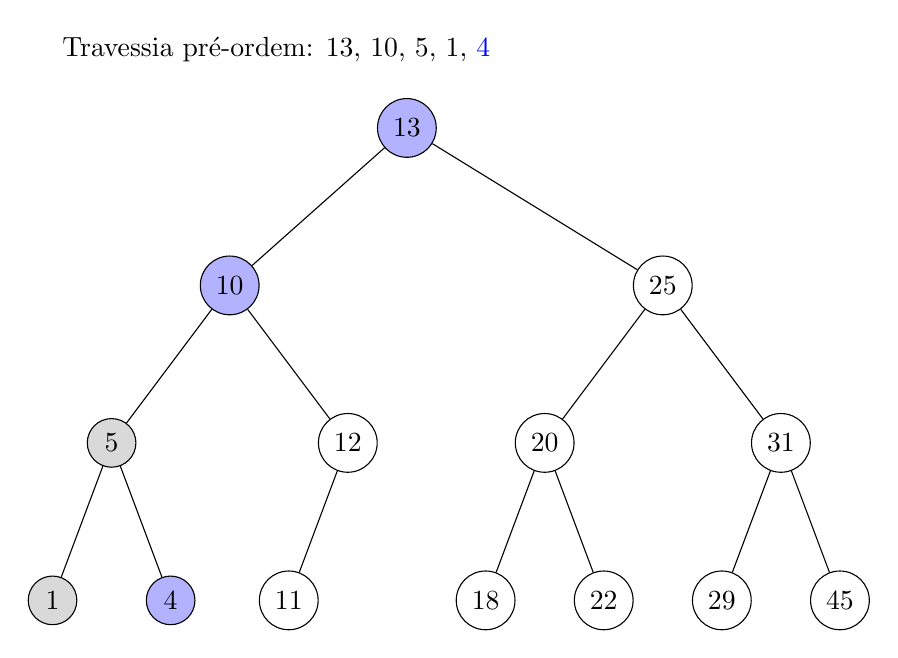
\begin{tikzpicture}

        \begin{scope}
            \node[anchor=west] (X) at (0, 6) { Travessia pré-ordem: 13, 10, 5, 1, \textcolor{blue}{4} };

            \node[circle,draw,fill=blue!30] (A) at (4.5, 5) { $13$ };
            \node[circle,draw,fill=blue!30] (B) at (2.25, 3) { $10$ };
            \node[circle,draw] (C) at (7.75, 3) { $25$ };
            \node[circle,draw,fill=gray!30] (D) at (0.75, 1) { $5$ };
            \node[circle,draw] (E) at (3.75, 1) { $12$ };
            \node[circle,draw] (F) at (6.25, 1) { $20$ };
            \node[circle,draw] (G) at (9.25, 1) { $31$ };
            \node[circle,draw,fill=gray!30] (H) at (0, -1) { $1$ };
            \node[circle,draw,fill=blue!30] (I) at (1.5, -1) { $4$ };
            \node[circle,draw] (J) at (3, -1) { $11$ };
            \node[circle,draw] (L) at (5.5, -1) { $18$ };
            \node[circle,draw] (M) at (7, -1) { $22$ };
            \node[circle,draw] (N) at (8.5, -1) { $29$ };
            \node[circle,draw] (O) at (10, -1) { $45$ };

            \draw (A) -- (B);
            \draw (A) -- (C);
            \draw (B) -- (D);
            \draw (B) -- (E);
            \draw (C) -- (F);
            \draw (C) -- (G);

            \draw (D) -- (H);
            \draw (D) -- (I);
            \draw (E) -- (J);
            \draw (F) -- (L);
            \draw (F) -- (M);
            \draw (G) -- (N);
            \draw (G) -- (O);
        \end{scope}
    \end{tikzpicture}

\end{frame}

\begin{frame}[fragile]{Exemplo de inserção em árvore binária de busca}

    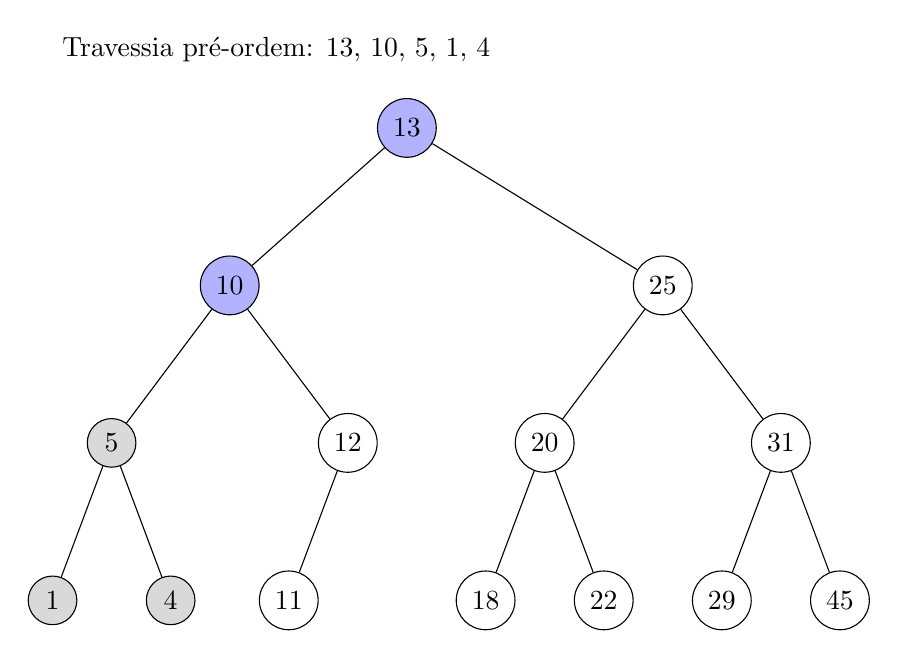
\begin{tikzpicture}

        \begin{scope}
            \node[anchor=west] (X) at (0, 6) { Travessia pré-ordem: 13, 10, 5, 1, 4\textcolor{blue}{} };

            \node[circle,draw,fill=blue!30] (A) at (4.5, 5) { $13$ };
            \node[circle,draw,fill=blue!30] (B) at (2.25, 3) { $10$ };
            \node[circle,draw] (C) at (7.75, 3) { $25$ };
            \node[circle,draw,fill=gray!30] (D) at (0.75, 1) { $5$ };
            \node[circle,draw] (E) at (3.75, 1) { $12$ };
            \node[circle,draw] (F) at (6.25, 1) { $20$ };
            \node[circle,draw] (G) at (9.25, 1) { $31$ };
            \node[circle,draw,fill=gray!30] (H) at (0, -1) { $1$ };
            \node[circle,draw,fill=gray!30] (I) at (1.5, -1) { $4$ };
            \node[circle,draw] (J) at (3, -1) { $11$ };
            \node[circle,draw] (L) at (5.5, -1) { $18$ };
            \node[circle,draw] (M) at (7, -1) { $22$ };
            \node[circle,draw] (N) at (8.5, -1) { $29$ };
            \node[circle,draw] (O) at (10, -1) { $45$ };

            \draw (A) -- (B);
            \draw (A) -- (C);
            \draw (B) -- (D);
            \draw (B) -- (E);
            \draw (C) -- (F);
            \draw (C) -- (G);

            \draw (D) -- (H);
            \draw (D) -- (I);
            \draw (E) -- (J);
            \draw (F) -- (L);
            \draw (F) -- (M);
            \draw (G) -- (N);
            \draw (G) -- (O);
        \end{scope}
    \end{tikzpicture}

\end{frame}

\begin{frame}[fragile]{Exemplo de inserção em árvore binária de busca}

    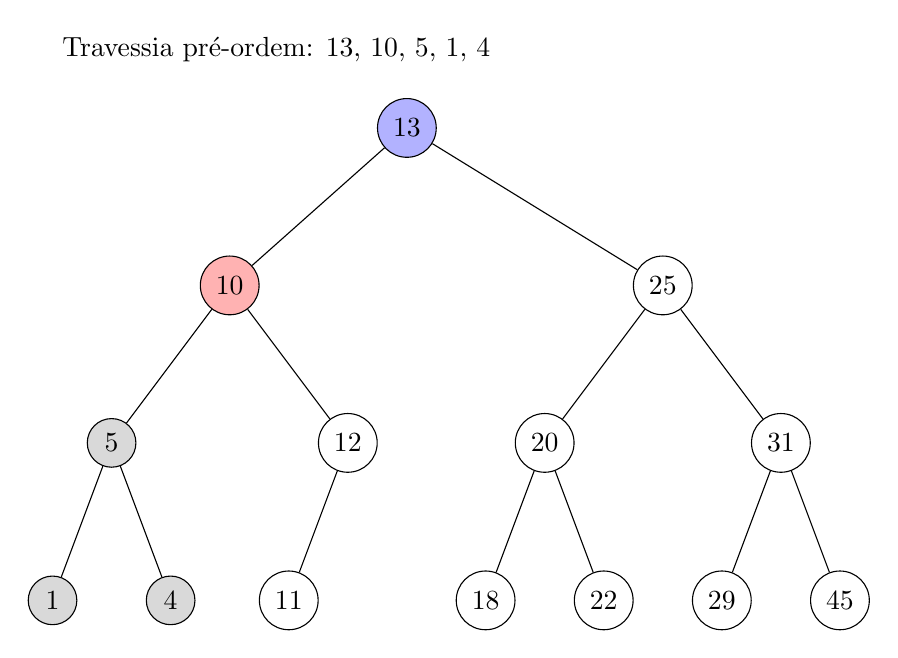
\begin{tikzpicture}

        \begin{scope}
            \node[anchor=west] (X) at (0, 6) { Travessia pré-ordem: 13, 10, 5, 1, 4\textcolor{blue}{} };

            \node[circle,draw,fill=blue!30] (A) at (4.5, 5) { $13$ };
            \node[circle,draw,fill=red!30] (B) at (2.25, 3) { $10$ };
            \node[circle,draw] (C) at (7.75, 3) { $25$ };
            \node[circle,draw,fill=gray!30] (D) at (0.75, 1) { $5$ };
            \node[circle,draw] (E) at (3.75, 1) { $12$ };
            \node[circle,draw] (F) at (6.25, 1) { $20$ };
            \node[circle,draw] (G) at (9.25, 1) { $31$ };
            \node[circle,draw,fill=gray!30] (H) at (0, -1) { $1$ };
            \node[circle,draw,fill=gray!30] (I) at (1.5, -1) { $4$ };
            \node[circle,draw] (J) at (3, -1) { $11$ };
            \node[circle,draw] (L) at (5.5, -1) { $18$ };
            \node[circle,draw] (M) at (7, -1) { $22$ };
            \node[circle,draw] (N) at (8.5, -1) { $29$ };
            \node[circle,draw] (O) at (10, -1) { $45$ };

            \draw (A) -- (B);
            \draw (A) -- (C);
            \draw (B) -- (D);
            \draw (B) -- (E);
            \draw (C) -- (F);
            \draw (C) -- (G);

            \draw (D) -- (H);
            \draw (D) -- (I);
            \draw (E) -- (J);
            \draw (F) -- (L);
            \draw (F) -- (M);
            \draw (G) -- (N);
            \draw (G) -- (O);
        \end{scope}
    \end{tikzpicture}

\end{frame}

\begin{frame}[fragile]{Exemplo de inserção em árvore binária de busca}

    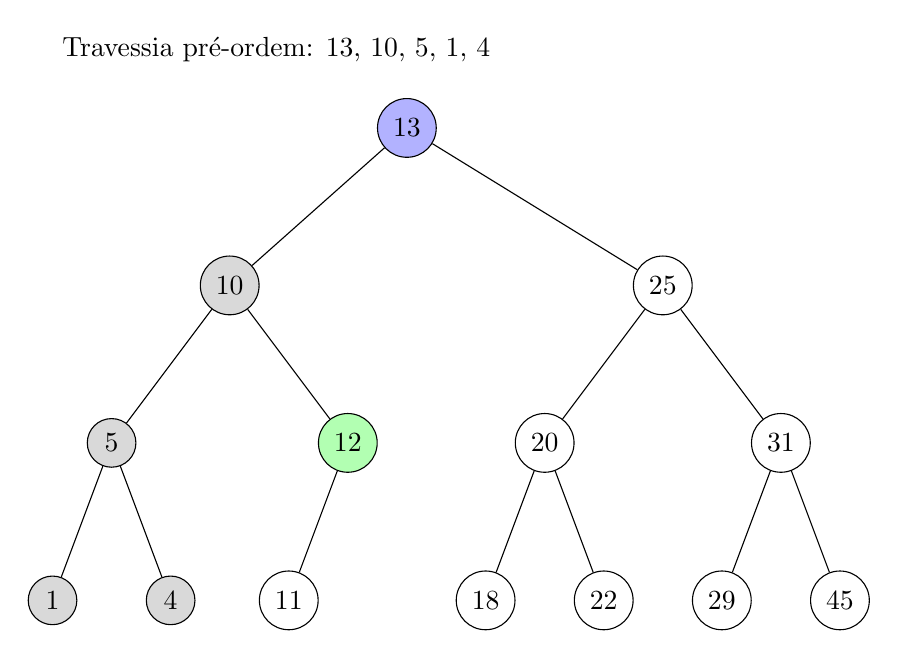
\begin{tikzpicture}

        \begin{scope}
            \node[anchor=west] (X) at (0, 6) { Travessia pré-ordem: 13, 10, 5, 1, 4\textcolor{blue}{} };

            \node[circle,draw,fill=blue!30] (A) at (4.5, 5) { $13$ };
            \node[circle,draw,fill=gray!30] (B) at (2.25, 3) { $10$ };
            \node[circle,draw] (C) at (7.75, 3) { $25$ };
            \node[circle,draw,fill=gray!30] (D) at (0.75, 1) { $5$ };
            \node[circle,draw,fill=green!30] (E) at (3.75, 1) { $12$ };
            \node[circle,draw] (F) at (6.25, 1) { $20$ };
            \node[circle,draw] (G) at (9.25, 1) { $31$ };
            \node[circle,draw,fill=gray!30] (H) at (0, -1) { $1$ };
            \node[circle,draw,fill=gray!30] (I) at (1.5, -1) { $4$ };
            \node[circle,draw] (J) at (3, -1) { $11$ };
            \node[circle,draw] (L) at (5.5, -1) { $18$ };
            \node[circle,draw] (M) at (7, -1) { $22$ };
            \node[circle,draw] (N) at (8.5, -1) { $29$ };
            \node[circle,draw] (O) at (10, -1) { $45$ };

            \draw (A) -- (B);
            \draw (A) -- (C);
            \draw (B) -- (D);
            \draw (B) -- (E);
            \draw (C) -- (F);
            \draw (C) -- (G);

            \draw (D) -- (H);
            \draw (D) -- (I);
            \draw (E) -- (J);
            \draw (F) -- (L);
            \draw (F) -- (M);
            \draw (G) -- (N);
            \draw (G) -- (O);
        \end{scope}
    \end{tikzpicture}

\end{frame}

\begin{frame}[fragile]{Exemplo de inserção em árvore binária de busca}

    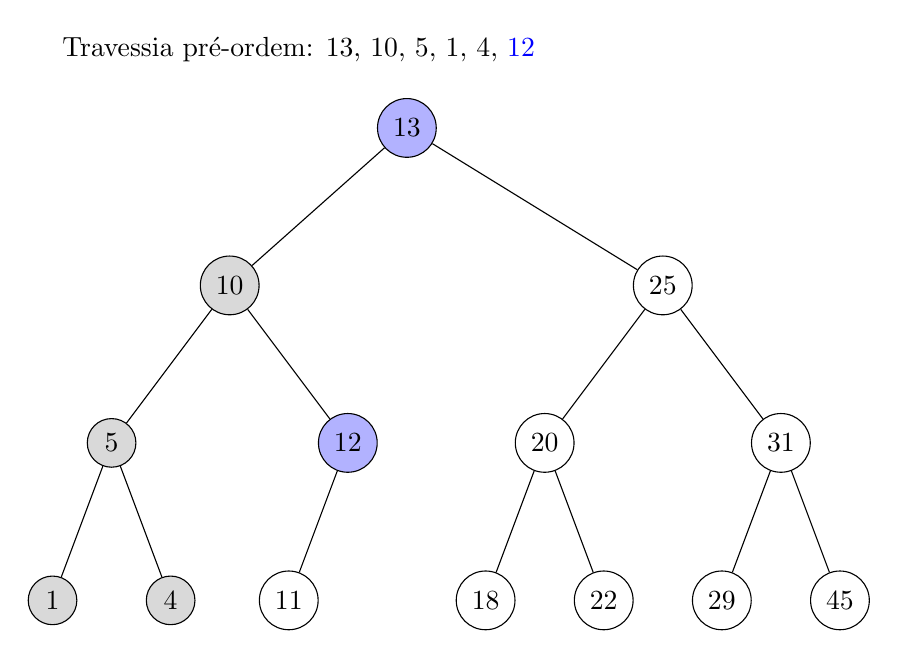
\begin{tikzpicture}

        \begin{scope}
            \node[anchor=west] (X) at (0, 6) { Travessia pré-ordem: 13, 10, 5, 1, 4, \textcolor{blue}{12} };

            \node[circle,draw,fill=blue!30] (A) at (4.5, 5) { $13$ };
            \node[circle,draw,fill=gray!30] (B) at (2.25, 3) { $10$ };
            \node[circle,draw] (C) at (7.75, 3) { $25$ };
            \node[circle,draw,fill=gray!30] (D) at (0.75, 1) { $5$ };
            \node[circle,draw,fill=blue!30] (E) at (3.75, 1) { $12$ };
            \node[circle,draw] (F) at (6.25, 1) { $20$ };
            \node[circle,draw] (G) at (9.25, 1) { $31$ };
            \node[circle,draw,fill=gray!30] (H) at (0, -1) { $1$ };
            \node[circle,draw,fill=gray!30] (I) at (1.5, -1) { $4$ };
            \node[circle,draw] (J) at (3, -1) { $11$ };
            \node[circle,draw] (L) at (5.5, -1) { $18$ };
            \node[circle,draw] (M) at (7, -1) { $22$ };
            \node[circle,draw] (N) at (8.5, -1) { $29$ };
            \node[circle,draw] (O) at (10, -1) { $45$ };

            \draw (A) -- (B);
            \draw (A) -- (C);
            \draw (B) -- (D);
            \draw (B) -- (E);
            \draw (C) -- (F);
            \draw (C) -- (G);

            \draw (D) -- (H);
            \draw (D) -- (I);
            \draw (E) -- (J);
            \draw (F) -- (L);
            \draw (F) -- (M);
            \draw (G) -- (N);
            \draw (G) -- (O);
        \end{scope}
    \end{tikzpicture}

\end{frame}

\begin{frame}[fragile]{Exemplo de inserção em árvore binária de busca}

    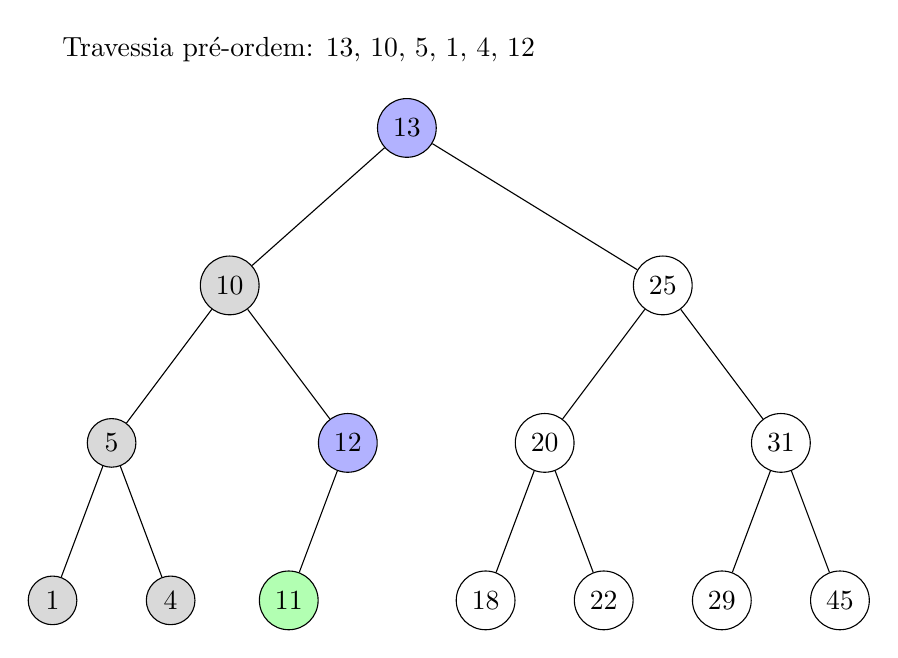
\begin{tikzpicture}

        \begin{scope}
            \node[anchor=west] (X) at (0, 6) { Travessia pré-ordem: 13, 10, 5, 1, 4, 12\textcolor{blue}{} };

            \node[circle,draw,fill=blue!30] (A) at (4.5, 5) { $13$ };
            \node[circle,draw,fill=gray!30] (B) at (2.25, 3) { $10$ };
            \node[circle,draw] (C) at (7.75, 3) { $25$ };
            \node[circle,draw,fill=gray!30] (D) at (0.75, 1) { $5$ };
            \node[circle,draw,fill=blue!30] (E) at (3.75, 1) { $12$ };
            \node[circle,draw] (F) at (6.25, 1) { $20$ };
            \node[circle,draw] (G) at (9.25, 1) { $31$ };
            \node[circle,draw,fill=gray!30] (H) at (0, -1) { $1$ };
            \node[circle,draw,fill=gray!30] (I) at (1.5, -1) { $4$ };
            \node[circle,draw,fill=green!30] (J) at (3, -1) { $11$ };
            \node[circle,draw] (L) at (5.5, -1) { $18$ };
            \node[circle,draw] (M) at (7, -1) { $22$ };
            \node[circle,draw] (N) at (8.5, -1) { $29$ };
            \node[circle,draw] (O) at (10, -1) { $45$ };

            \draw (A) -- (B);
            \draw (A) -- (C);
            \draw (B) -- (D);
            \draw (B) -- (E);
            \draw (C) -- (F);
            \draw (C) -- (G);

            \draw (D) -- (H);
            \draw (D) -- (I);
            \draw (E) -- (J);
            \draw (F) -- (L);
            \draw (F) -- (M);
            \draw (G) -- (N);
            \draw (G) -- (O);
        \end{scope}
    \end{tikzpicture}

\end{frame}

\begin{frame}[fragile]{Exemplo de inserção em árvore binária de busca}

    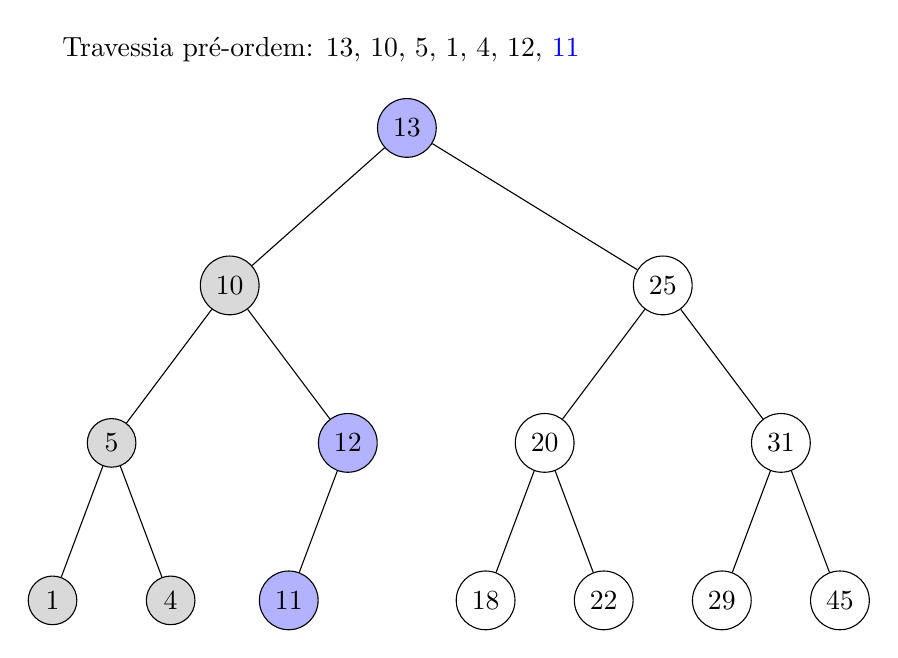
\begin{tikzpicture}

        \begin{scope}
            \node[anchor=west] (X) at (0, 6) { Travessia pré-ordem: 13, 10, 5, 1, 4, 12, \textcolor{blue}{11} };

            \node[circle,draw,fill=blue!30] (A) at (4.5, 5) { $13$ };
            \node[circle,draw,fill=gray!30] (B) at (2.25, 3) { $10$ };
            \node[circle,draw] (C) at (7.75, 3) { $25$ };
            \node[circle,draw,fill=gray!30] (D) at (0.75, 1) { $5$ };
            \node[circle,draw,fill=blue!30] (E) at (3.75, 1) { $12$ };
            \node[circle,draw] (F) at (6.25, 1) { $20$ };
            \node[circle,draw] (G) at (9.25, 1) { $31$ };
            \node[circle,draw,fill=gray!30] (H) at (0, -1) { $1$ };
            \node[circle,draw,fill=gray!30] (I) at (1.5, -1) { $4$ };
            \node[circle,draw,fill=blue!30] (J) at (3, -1) { $11$ };
            \node[circle,draw] (L) at (5.5, -1) { $18$ };
            \node[circle,draw] (M) at (7, -1) { $22$ };
            \node[circle,draw] (N) at (8.5, -1) { $29$ };
            \node[circle,draw] (O) at (10, -1) { $45$ };

            \draw (A) -- (B);
            \draw (A) -- (C);
            \draw (B) -- (D);
            \draw (B) -- (E);
            \draw (C) -- (F);
            \draw (C) -- (G);

            \draw (D) -- (H);
            \draw (D) -- (I);
            \draw (E) -- (J);
            \draw (F) -- (L);
            \draw (F) -- (M);
            \draw (G) -- (N);
            \draw (G) -- (O);
        \end{scope}
    \end{tikzpicture}

\end{frame}

\begin{frame}[fragile]{Exemplo de inserção em árvore binária de busca}

    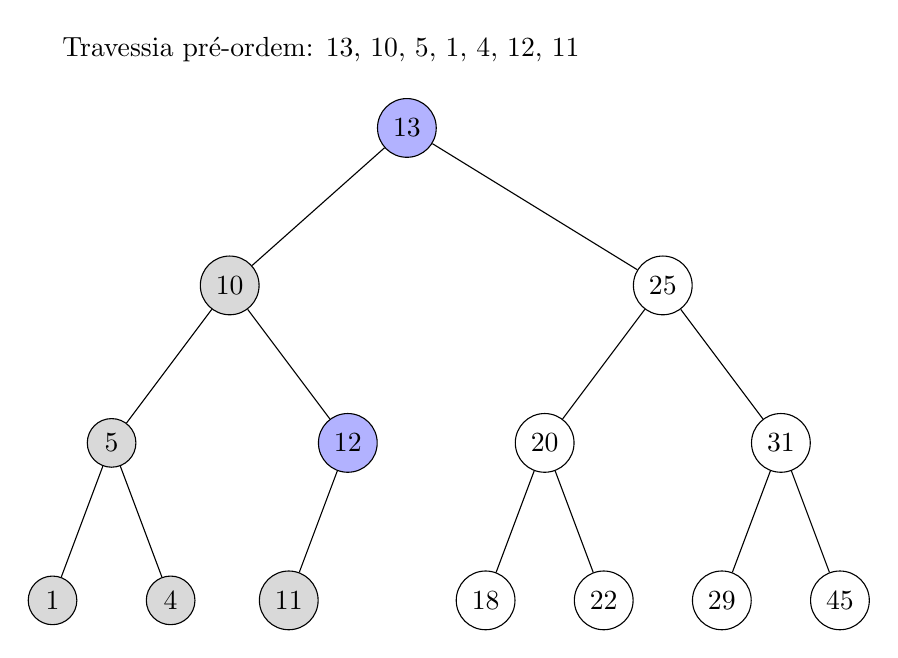
\begin{tikzpicture}

        \begin{scope}
            \node[anchor=west] (X) at (0, 6) { Travessia pré-ordem: 13, 10, 5, 1, 4, 12, 11\textcolor{blue}{} };

            \node[circle,draw,fill=blue!30] (A) at (4.5, 5) { $13$ };
            \node[circle,draw,fill=gray!30] (B) at (2.25, 3) { $10$ };
            \node[circle,draw] (C) at (7.75, 3) { $25$ };
            \node[circle,draw,fill=gray!30] (D) at (0.75, 1) { $5$ };
            \node[circle,draw,fill=blue!30] (E) at (3.75, 1) { $12$ };
            \node[circle,draw] (F) at (6.25, 1) { $20$ };
            \node[circle,draw] (G) at (9.25, 1) { $31$ };
            \node[circle,draw,fill=gray!30] (H) at (0, -1) { $1$ };
            \node[circle,draw,fill=gray!30] (I) at (1.5, -1) { $4$ };
            \node[circle,draw,fill=gray!30] (J) at (3, -1) { $11$ };
            \node[circle,draw] (L) at (5.5, -1) { $18$ };
            \node[circle,draw] (M) at (7, -1) { $22$ };
            \node[circle,draw] (N) at (8.5, -1) { $29$ };
            \node[circle,draw] (O) at (10, -1) { $45$ };

            \draw (A) -- (B);
            \draw (A) -- (C);
            \draw (B) -- (D);
            \draw (B) -- (E);
            \draw (C) -- (F);
            \draw (C) -- (G);

            \draw (D) -- (H);
            \draw (D) -- (I);
            \draw (E) -- (J);
            \draw (F) -- (L);
            \draw (F) -- (M);
            \draw (G) -- (N);
            \draw (G) -- (O);
        \end{scope}
    \end{tikzpicture}

\end{frame}

\begin{frame}[fragile]{Exemplo de inserção em árvore binária de busca}

    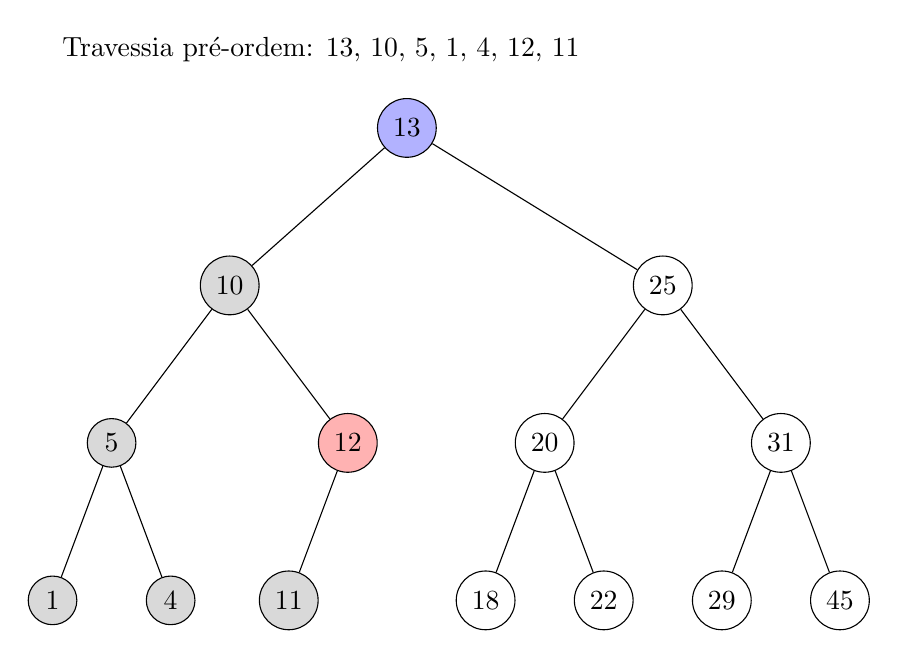
\begin{tikzpicture}

        \begin{scope}
            \node[anchor=west] (X) at (0, 6) { Travessia pré-ordem: 13, 10, 5, 1, 4, 12, 11\textcolor{blue}{} };

            \node[circle,draw,fill=blue!30] (A) at (4.5, 5) { $13$ };
            \node[circle,draw,fill=gray!30] (B) at (2.25, 3) { $10$ };
            \node[circle,draw] (C) at (7.75, 3) { $25$ };
            \node[circle,draw,fill=gray!30] (D) at (0.75, 1) { $5$ };
            \node[circle,draw,fill=red!30] (E) at (3.75, 1) { $12$ };
            \node[circle,draw] (F) at (6.25, 1) { $20$ };
            \node[circle,draw] (G) at (9.25, 1) { $31$ };
            \node[circle,draw,fill=gray!30] (H) at (0, -1) { $1$ };
            \node[circle,draw,fill=gray!30] (I) at (1.5, -1) { $4$ };
            \node[circle,draw,fill=gray!30] (J) at (3, -1) { $11$ };
            \node[circle,draw] (L) at (5.5, -1) { $18$ };
            \node[circle,draw] (M) at (7, -1) { $22$ };
            \node[circle,draw] (N) at (8.5, -1) { $29$ };
            \node[circle,draw] (O) at (10, -1) { $45$ };

            \draw (A) -- (B);
            \draw (A) -- (C);
            \draw (B) -- (D);
            \draw (B) -- (E);
            \draw (C) -- (F);
            \draw (C) -- (G);

            \draw (D) -- (H);
            \draw (D) -- (I);
            \draw (E) -- (J);
            \draw (F) -- (L);
            \draw (F) -- (M);
            \draw (G) -- (N);
            \draw (G) -- (O);
        \end{scope}
    \end{tikzpicture}

\end{frame}

\begin{frame}[fragile]{Exemplo de inserção em árvore binária de busca}

    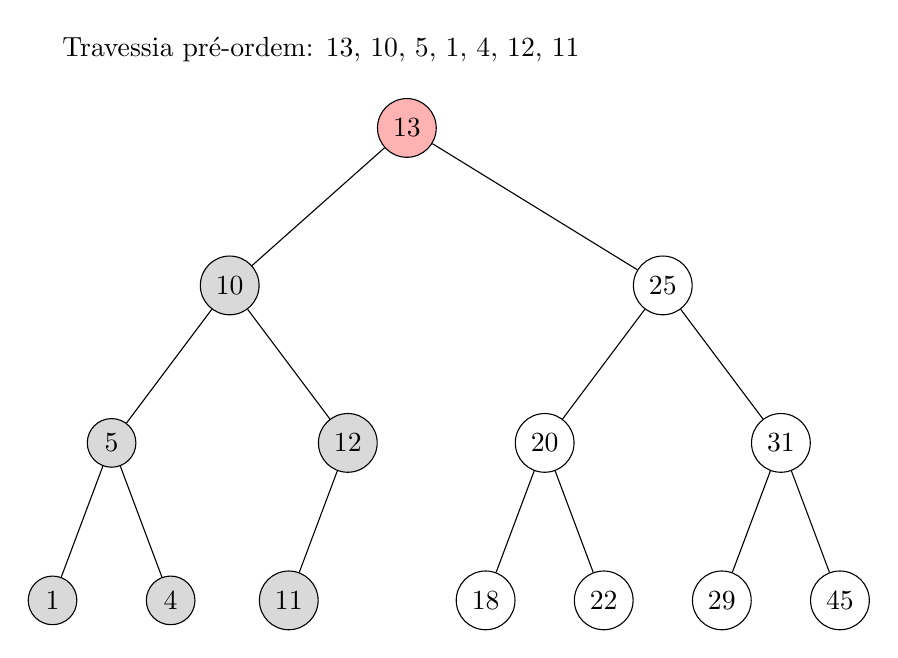
\begin{tikzpicture}

        \begin{scope}
            \node[anchor=west] (X) at (0, 6) { Travessia pré-ordem: 13, 10, 5, 1, 4, 12, 11\textcolor{blue}{} };

            \node[circle,draw,fill=red!30] (A) at (4.5, 5) { $13$ };
            \node[circle,draw,fill=gray!30] (B) at (2.25, 3) { $10$ };
            \node[circle,draw] (C) at (7.75, 3) { $25$ };
            \node[circle,draw,fill=gray!30] (D) at (0.75, 1) { $5$ };
            \node[circle,draw,fill=gray!30] (E) at (3.75, 1) { $12$ };
            \node[circle,draw] (F) at (6.25, 1) { $20$ };
            \node[circle,draw] (G) at (9.25, 1) { $31$ };
            \node[circle,draw,fill=gray!30] (H) at (0, -1) { $1$ };
            \node[circle,draw,fill=gray!30] (I) at (1.5, -1) { $4$ };
            \node[circle,draw,fill=gray!30] (J) at (3, -1) { $11$ };
            \node[circle,draw] (L) at (5.5, -1) { $18$ };
            \node[circle,draw] (M) at (7, -1) { $22$ };
            \node[circle,draw] (N) at (8.5, -1) { $29$ };
            \node[circle,draw] (O) at (10, -1) { $45$ };

            \draw (A) -- (B);
            \draw (A) -- (C);
            \draw (B) -- (D);
            \draw (B) -- (E);
            \draw (C) -- (F);
            \draw (C) -- (G);

            \draw (D) -- (H);
            \draw (D) -- (I);
            \draw (E) -- (J);
            \draw (F) -- (L);
            \draw (F) -- (M);
            \draw (G) -- (N);
            \draw (G) -- (O);
        \end{scope}
    \end{tikzpicture}

\end{frame}

\begin{frame}[fragile]{Exemplo de inserção em árvore binária de busca}

    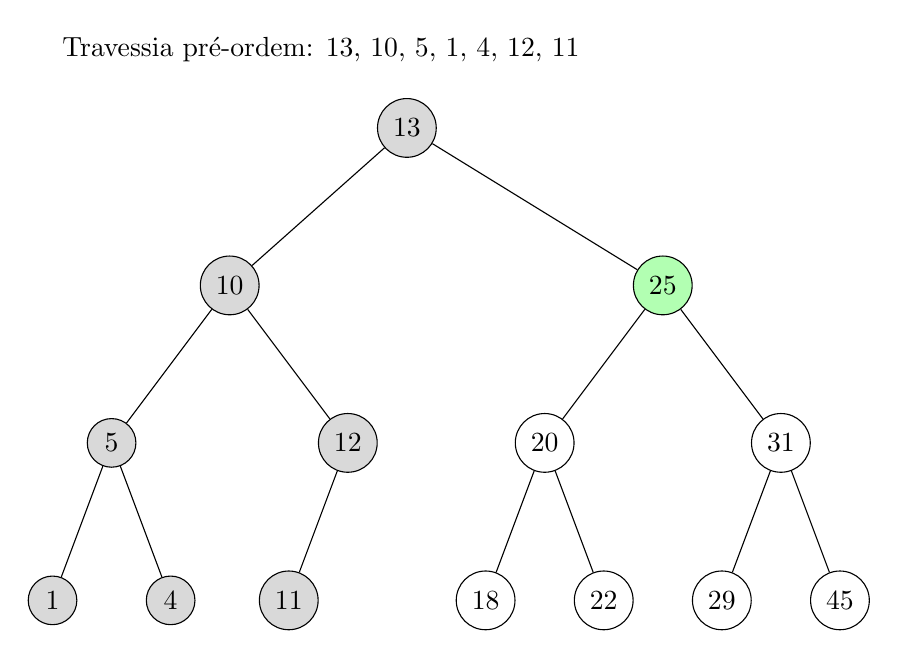
\begin{tikzpicture}

        \begin{scope}
            \node[anchor=west] (X) at (0, 6) { Travessia pré-ordem: 13, 10, 5, 1, 4, 12, 11\textcolor{blue}{} };

            \node[circle,draw,fill=gray!30] (A) at (4.5, 5) { $13$ };
            \node[circle,draw,fill=gray!30] (B) at (2.25, 3) { $10$ };
            \node[circle,draw,fill=green!30] (C) at (7.75, 3) { $25$ };
            \node[circle,draw,fill=gray!30] (D) at (0.75, 1) { $5$ };
            \node[circle,draw,fill=gray!30] (E) at (3.75, 1) { $12$ };
            \node[circle,draw] (F) at (6.25, 1) { $20$ };
            \node[circle,draw] (G) at (9.25, 1) { $31$ };
            \node[circle,draw,fill=gray!30] (H) at (0, -1) { $1$ };
            \node[circle,draw,fill=gray!30] (I) at (1.5, -1) { $4$ };
            \node[circle,draw,fill=gray!30] (J) at (3, -1) { $11$ };
            \node[circle,draw] (L) at (5.5, -1) { $18$ };
            \node[circle,draw] (M) at (7, -1) { $22$ };
            \node[circle,draw] (N) at (8.5, -1) { $29$ };
            \node[circle,draw] (O) at (10, -1) { $45$ };

            \draw (A) -- (B);
            \draw (A) -- (C);
            \draw (B) -- (D);
            \draw (B) -- (E);
            \draw (C) -- (F);
            \draw (C) -- (G);

            \draw (D) -- (H);
            \draw (D) -- (I);
            \draw (E) -- (J);
            \draw (F) -- (L);
            \draw (F) -- (M);
            \draw (G) -- (N);
            \draw (G) -- (O);
        \end{scope}
    \end{tikzpicture}

\end{frame}

\begin{frame}[fragile]{Exemplo de inserção em árvore binária de busca}

    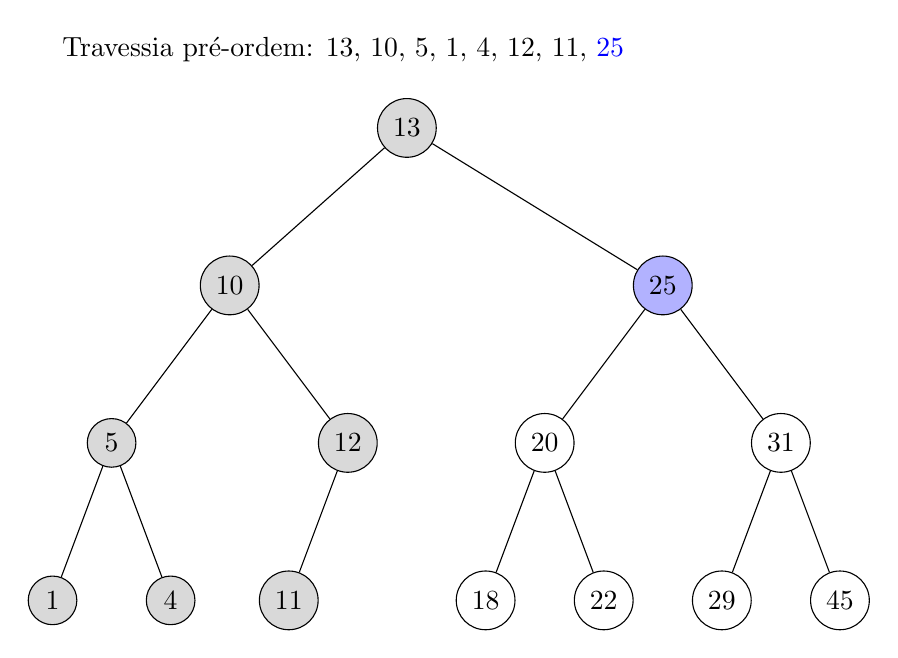
\begin{tikzpicture}

        \begin{scope}
            \node[anchor=west] (X) at (0, 6) { Travessia pré-ordem: 13, 10, 5, 1, 4, 12, 11, \textcolor{blue}{25} };

            \node[circle,draw,fill=gray!30] (A) at (4.5, 5) { $13$ };
            \node[circle,draw,fill=gray!30] (B) at (2.25, 3) { $10$ };
            \node[circle,draw,fill=blue!30] (C) at (7.75, 3) { $25$ };
            \node[circle,draw,fill=gray!30] (D) at (0.75, 1) { $5$ };
            \node[circle,draw,fill=gray!30] (E) at (3.75, 1) { $12$ };
            \node[circle,draw] (F) at (6.25, 1) { $20$ };
            \node[circle,draw] (G) at (9.25, 1) { $31$ };
            \node[circle,draw,fill=gray!30] (H) at (0, -1) { $1$ };
            \node[circle,draw,fill=gray!30] (I) at (1.5, -1) { $4$ };
            \node[circle,draw,fill=gray!30] (J) at (3, -1) { $11$ };
            \node[circle,draw] (L) at (5.5, -1) { $18$ };
            \node[circle,draw] (M) at (7, -1) { $22$ };
            \node[circle,draw] (N) at (8.5, -1) { $29$ };
            \node[circle,draw] (O) at (10, -1) { $45$ };

            \draw (A) -- (B);
            \draw (A) -- (C);
            \draw (B) -- (D);
            \draw (B) -- (E);
            \draw (C) -- (F);
            \draw (C) -- (G);

            \draw (D) -- (H);
            \draw (D) -- (I);
            \draw (E) -- (J);
            \draw (F) -- (L);
            \draw (F) -- (M);
            \draw (G) -- (N);
            \draw (G) -- (O);
        \end{scope}
    \end{tikzpicture}

\end{frame}

\begin{frame}[fragile]{Exemplo de inserção em árvore binária de busca}

    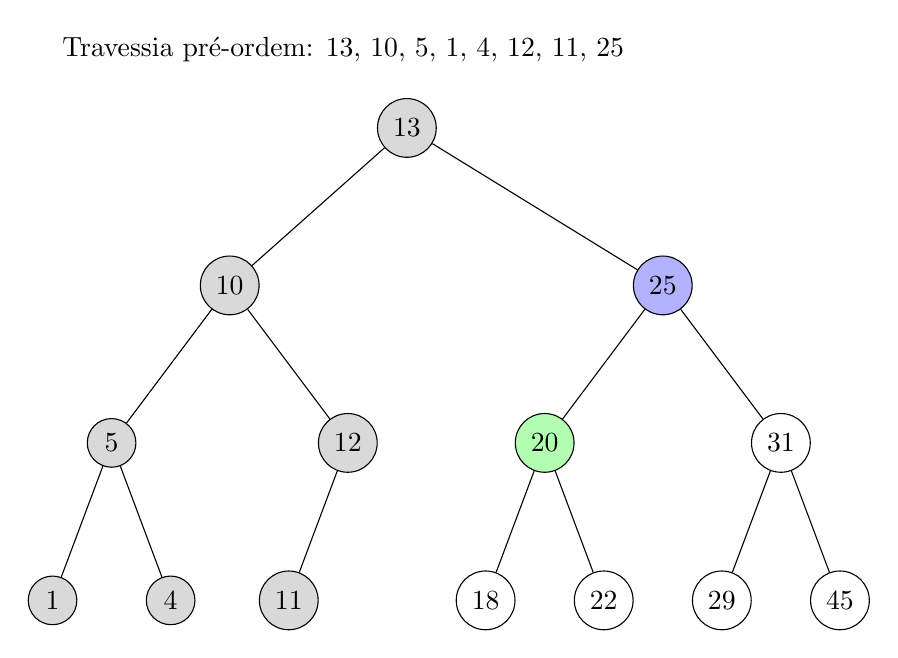
\begin{tikzpicture}

        \begin{scope}
            \node[anchor=west] (X) at (0, 6) { Travessia pré-ordem: 13, 10, 5, 1, 4, 12, 11, 25\textcolor{blue}{} };

            \node[circle,draw,fill=gray!30] (A) at (4.5, 5) { $13$ };
            \node[circle,draw,fill=gray!30] (B) at (2.25, 3) { $10$ };
            \node[circle,draw,fill=blue!30] (C) at (7.75, 3) { $25$ };
            \node[circle,draw,fill=gray!30] (D) at (0.75, 1) { $5$ };
            \node[circle,draw,fill=gray!30] (E) at (3.75, 1) { $12$ };
            \node[circle,draw,fill=green!30] (F) at (6.25, 1) { $20$ };
            \node[circle,draw] (G) at (9.25, 1) { $31$ };
            \node[circle,draw,fill=gray!30] (H) at (0, -1) { $1$ };
            \node[circle,draw,fill=gray!30] (I) at (1.5, -1) { $4$ };
            \node[circle,draw,fill=gray!30] (J) at (3, -1) { $11$ };
            \node[circle,draw] (L) at (5.5, -1) { $18$ };
            \node[circle,draw] (M) at (7, -1) { $22$ };
            \node[circle,draw] (N) at (8.5, -1) { $29$ };
            \node[circle,draw] (O) at (10, -1) { $45$ };

            \draw (A) -- (B);
            \draw (A) -- (C);
            \draw (B) -- (D);
            \draw (B) -- (E);
            \draw (C) -- (F);
            \draw (C) -- (G);

            \draw (D) -- (H);
            \draw (D) -- (I);
            \draw (E) -- (J);
            \draw (F) -- (L);
            \draw (F) -- (M);
            \draw (G) -- (N);
            \draw (G) -- (O);
        \end{scope}
    \end{tikzpicture}

\end{frame}

\begin{frame}[fragile]{Exemplo de inserção em árvore binária de busca}

    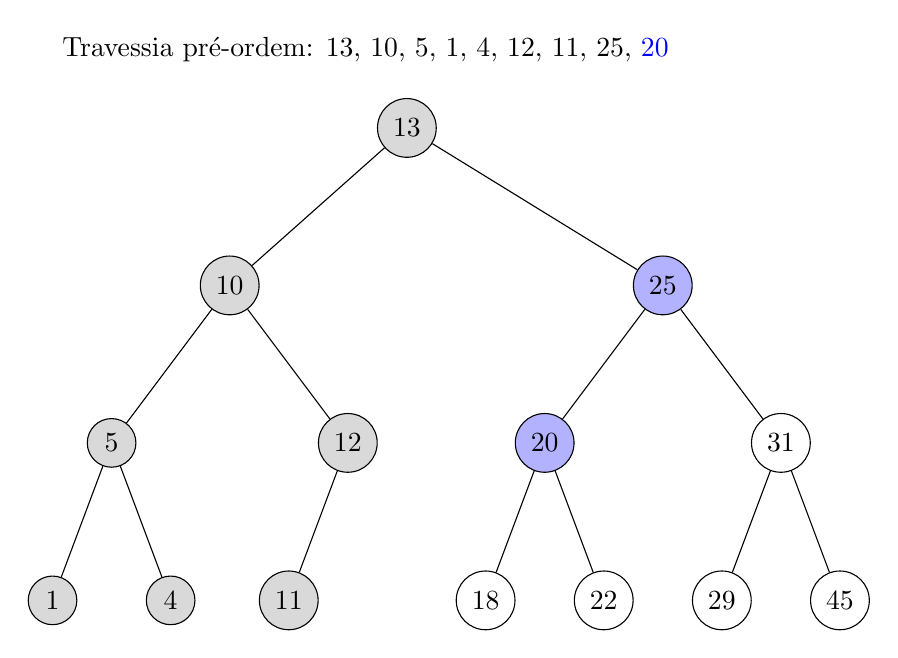
\begin{tikzpicture}

        \begin{scope}
            \node[anchor=west] (X) at (0, 6) { Travessia pré-ordem: 13, 10, 5, 1, 4, 12, 11, 25, \textcolor{blue}{20} };

            \node[circle,draw,fill=gray!30] (A) at (4.5, 5) { $13$ };
            \node[circle,draw,fill=gray!30] (B) at (2.25, 3) { $10$ };
            \node[circle,draw,fill=blue!30] (C) at (7.75, 3) { $25$ };
            \node[circle,draw,fill=gray!30] (D) at (0.75, 1) { $5$ };
            \node[circle,draw,fill=gray!30] (E) at (3.75, 1) { $12$ };
            \node[circle,draw,fill=blue!30] (F) at (6.25, 1) { $20$ };
            \node[circle,draw] (G) at (9.25, 1) { $31$ };
            \node[circle,draw,fill=gray!30] (H) at (0, -1) { $1$ };
            \node[circle,draw,fill=gray!30] (I) at (1.5, -1) { $4$ };
            \node[circle,draw,fill=gray!30] (J) at (3, -1) { $11$ };
            \node[circle,draw] (L) at (5.5, -1) { $18$ };
            \node[circle,draw] (M) at (7, -1) { $22$ };
            \node[circle,draw] (N) at (8.5, -1) { $29$ };
            \node[circle,draw] (O) at (10, -1) { $45$ };

            \draw (A) -- (B);
            \draw (A) -- (C);
            \draw (B) -- (D);
            \draw (B) -- (E);
            \draw (C) -- (F);
            \draw (C) -- (G);

            \draw (D) -- (H);
            \draw (D) -- (I);
            \draw (E) -- (J);
            \draw (F) -- (L);
            \draw (F) -- (M);
            \draw (G) -- (N);
            \draw (G) -- (O);
        \end{scope}
    \end{tikzpicture}

\end{frame}

\begin{frame}[fragile]{Exemplo de inserção em árvore binária de busca}

    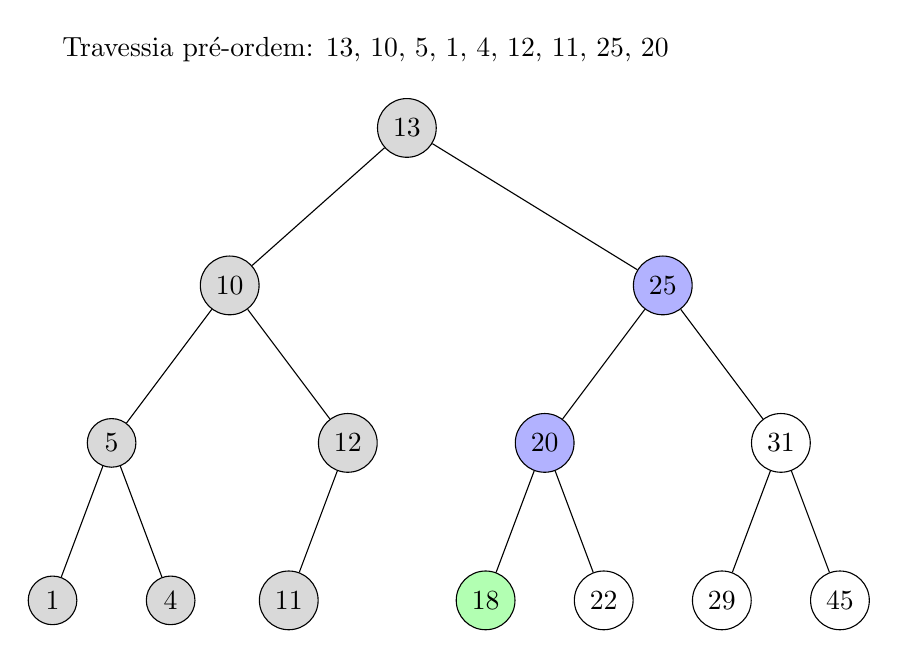
\begin{tikzpicture}

        \begin{scope}
            \node[anchor=west] (X) at (0, 6) { Travessia pré-ordem: 13, 10, 5, 1, 4, 12, 11, 25, 20 \textcolor{blue}{} };

            \node[circle,draw,fill=gray!30] (A) at (4.5, 5) { $13$ };
            \node[circle,draw,fill=gray!30] (B) at (2.25, 3) { $10$ };
            \node[circle,draw,fill=blue!30] (C) at (7.75, 3) { $25$ };
            \node[circle,draw,fill=gray!30] (D) at (0.75, 1) { $5$ };
            \node[circle,draw,fill=gray!30] (E) at (3.75, 1) { $12$ };
            \node[circle,draw,fill=blue!30] (F) at (6.25, 1) { $20$ };
            \node[circle,draw] (G) at (9.25, 1) { $31$ };
            \node[circle,draw,fill=gray!30] (H) at (0, -1) { $1$ };
            \node[circle,draw,fill=gray!30] (I) at (1.5, -1) { $4$ };
            \node[circle,draw,fill=gray!30] (J) at (3, -1) { $11$ };
            \node[circle,draw,fill=green!30] (L) at (5.5, -1) { $18$ };
            \node[circle,draw] (M) at (7, -1) { $22$ };
            \node[circle,draw] (N) at (8.5, -1) { $29$ };
            \node[circle,draw] (O) at (10, -1) { $45$ };

            \draw (A) -- (B);
            \draw (A) -- (C);
            \draw (B) -- (D);
            \draw (B) -- (E);
            \draw (C) -- (F);
            \draw (C) -- (G);

            \draw (D) -- (H);
            \draw (D) -- (I);
            \draw (E) -- (J);
            \draw (F) -- (L);
            \draw (F) -- (M);
            \draw (G) -- (N);
            \draw (G) -- (O);
        \end{scope}
    \end{tikzpicture}

\end{frame}

\begin{frame}[fragile]{Exemplo de inserção em árvore binária de busca}

    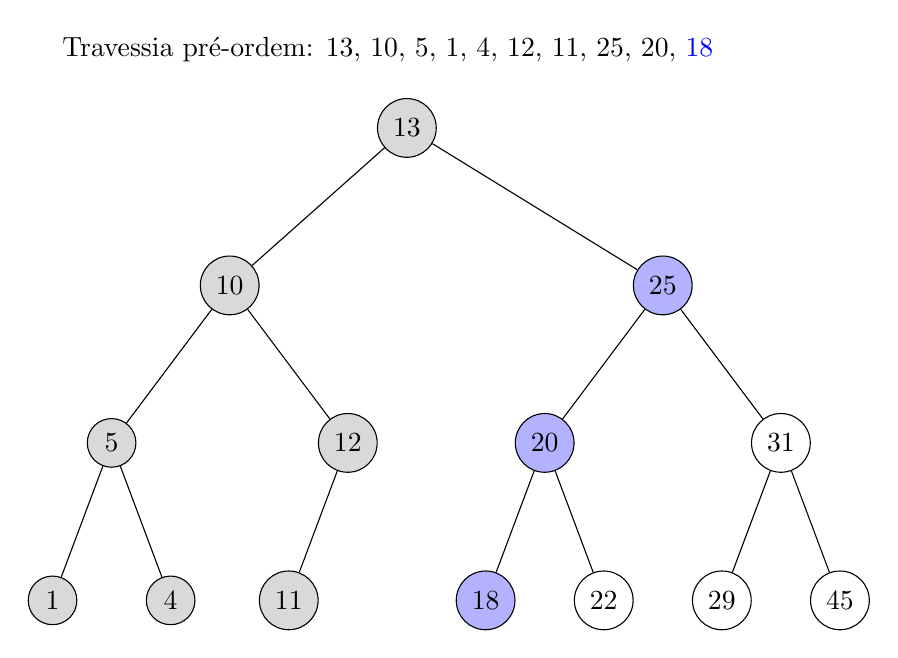
\begin{tikzpicture}

        \begin{scope}
            \node[anchor=west] (X) at (0, 6) { Travessia pré-ordem: 13, 10, 5, 1, 4, 12, 11, 25, 20, \textcolor{blue}{18} };

            \node[circle,draw,fill=gray!30] (A) at (4.5, 5) { $13$ };
            \node[circle,draw,fill=gray!30] (B) at (2.25, 3) { $10$ };
            \node[circle,draw,fill=blue!30] (C) at (7.75, 3) { $25$ };
            \node[circle,draw,fill=gray!30] (D) at (0.75, 1) { $5$ };
            \node[circle,draw,fill=gray!30] (E) at (3.75, 1) { $12$ };
            \node[circle,draw,fill=blue!30] (F) at (6.25, 1) { $20$ };
            \node[circle,draw] (G) at (9.25, 1) { $31$ };
            \node[circle,draw,fill=gray!30] (H) at (0, -1) { $1$ };
            \node[circle,draw,fill=gray!30] (I) at (1.5, -1) { $4$ };
            \node[circle,draw,fill=gray!30] (J) at (3, -1) { $11$ };
            \node[circle,draw,fill=blue!30] (L) at (5.5, -1) { $18$ };
            \node[circle,draw] (M) at (7, -1) { $22$ };
            \node[circle,draw] (N) at (8.5, -1) { $29$ };
            \node[circle,draw] (O) at (10, -1) { $45$ };

            \draw (A) -- (B);
            \draw (A) -- (C);
            \draw (B) -- (D);
            \draw (B) -- (E);
            \draw (C) -- (F);
            \draw (C) -- (G);

            \draw (D) -- (H);
            \draw (D) -- (I);
            \draw (E) -- (J);
            \draw (F) -- (L);
            \draw (F) -- (M);
            \draw (G) -- (N);
            \draw (G) -- (O);
        \end{scope}
    \end{tikzpicture}

\end{frame}

\begin{frame}[fragile]{Exemplo de inserção em árvore binária de busca}

    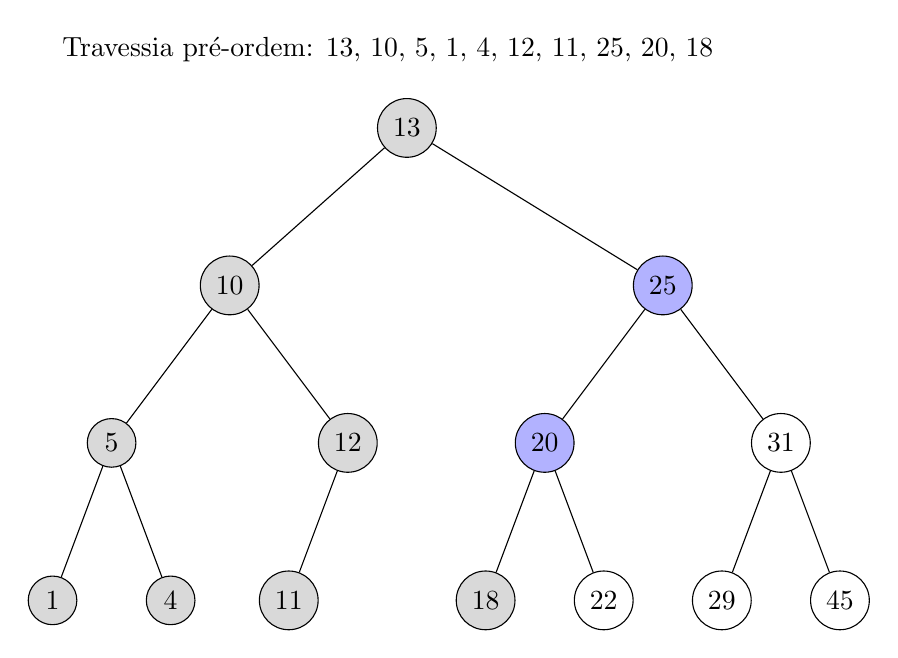
\begin{tikzpicture}

        \begin{scope}
            \node[anchor=west] (X) at (0, 6) { Travessia pré-ordem: 13, 10, 5, 1, 4, 12, 11, 25, 20, 18 \textcolor{blue}{} };

            \node[circle,draw,fill=gray!30] (A) at (4.5, 5) { $13$ };
            \node[circle,draw,fill=gray!30] (B) at (2.25, 3) { $10$ };
            \node[circle,draw,fill=blue!30] (C) at (7.75, 3) { $25$ };
            \node[circle,draw,fill=gray!30] (D) at (0.75, 1) { $5$ };
            \node[circle,draw,fill=gray!30] (E) at (3.75, 1) { $12$ };
            \node[circle,draw,fill=blue!30] (F) at (6.25, 1) { $20$ };
            \node[circle,draw] (G) at (9.25, 1) { $31$ };
            \node[circle,draw,fill=gray!30] (H) at (0, -1) { $1$ };
            \node[circle,draw,fill=gray!30] (I) at (1.5, -1) { $4$ };
            \node[circle,draw,fill=gray!30] (J) at (3, -1) { $11$ };
            \node[circle,draw,fill=gray!30] (L) at (5.5, -1) { $18$ };
            \node[circle,draw] (M) at (7, -1) { $22$ };
            \node[circle,draw] (N) at (8.5, -1) { $29$ };
            \node[circle,draw] (O) at (10, -1) { $45$ };

            \draw (A) -- (B);
            \draw (A) -- (C);
            \draw (B) -- (D);
            \draw (B) -- (E);
            \draw (C) -- (F);
            \draw (C) -- (G);

            \draw (D) -- (H);
            \draw (D) -- (I);
            \draw (E) -- (J);
            \draw (F) -- (L);
            \draw (F) -- (M);
            \draw (G) -- (N);
            \draw (G) -- (O);
        \end{scope}
    \end{tikzpicture}

\end{frame}

\begin{frame}[fragile]{Exemplo de inserção em árvore binária de busca}

    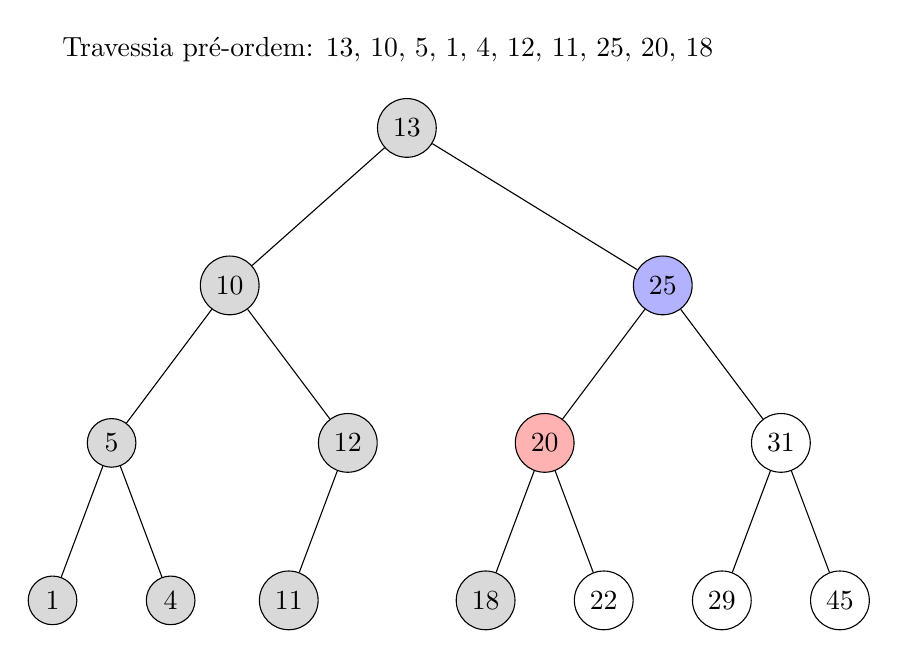
\begin{tikzpicture}

        \begin{scope}
            \node[anchor=west] (X) at (0, 6) { Travessia pré-ordem: 13, 10, 5, 1, 4, 12, 11, 25, 20, 18 \textcolor{blue}{} };

            \node[circle,draw,fill=gray!30] (A) at (4.5, 5) { $13$ };
            \node[circle,draw,fill=gray!30] (B) at (2.25, 3) { $10$ };
            \node[circle,draw,fill=blue!30] (C) at (7.75, 3) { $25$ };
            \node[circle,draw,fill=gray!30] (D) at (0.75, 1) { $5$ };
            \node[circle,draw,fill=gray!30] (E) at (3.75, 1) { $12$ };
            \node[circle,draw,fill=red!30] (F) at (6.25, 1) { $20$ };
            \node[circle,draw] (G) at (9.25, 1) { $31$ };
            \node[circle,draw,fill=gray!30] (H) at (0, -1) { $1$ };
            \node[circle,draw,fill=gray!30] (I) at (1.5, -1) { $4$ };
            \node[circle,draw,fill=gray!30] (J) at (3, -1) { $11$ };
            \node[circle,draw,fill=gray!30] (L) at (5.5, -1) { $18$ };
            \node[circle,draw] (M) at (7, -1) { $22$ };
            \node[circle,draw] (N) at (8.5, -1) { $29$ };
            \node[circle,draw] (O) at (10, -1) { $45$ };

            \draw (A) -- (B);
            \draw (A) -- (C);
            \draw (B) -- (D);
            \draw (B) -- (E);
            \draw (C) -- (F);
            \draw (C) -- (G);

            \draw (D) -- (H);
            \draw (D) -- (I);
            \draw (E) -- (J);
            \draw (F) -- (L);
            \draw (F) -- (M);
            \draw (G) -- (N);
            \draw (G) -- (O);
        \end{scope}
    \end{tikzpicture}

\end{frame}

\begin{frame}[fragile]{Exemplo de inserção em árvore binária de busca}

    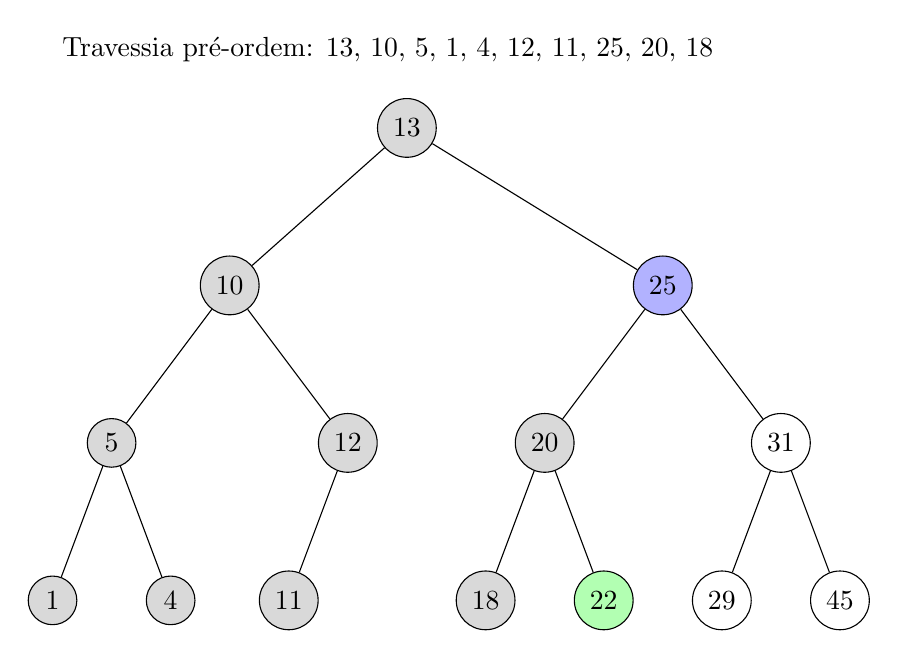
\begin{tikzpicture}

        \begin{scope}
            \node[anchor=west] (X) at (0, 6) { Travessia pré-ordem: 13, 10, 5, 1, 4, 12, 11, 25, 20, 18 \textcolor{blue}{} };

            \node[circle,draw,fill=gray!30] (A) at (4.5, 5) { $13$ };
            \node[circle,draw,fill=gray!30] (B) at (2.25, 3) { $10$ };
            \node[circle,draw,fill=blue!30] (C) at (7.75, 3) { $25$ };
            \node[circle,draw,fill=gray!30] (D) at (0.75, 1) { $5$ };
            \node[circle,draw,fill=gray!30] (E) at (3.75, 1) { $12$ };
            \node[circle,draw,fill=gray!30] (F) at (6.25, 1) { $20$ };
            \node[circle,draw] (G) at (9.25, 1) { $31$ };
            \node[circle,draw,fill=gray!30] (H) at (0, -1) { $1$ };
            \node[circle,draw,fill=gray!30] (I) at (1.5, -1) { $4$ };
            \node[circle,draw,fill=gray!30] (J) at (3, -1) { $11$ };
            \node[circle,draw,fill=gray!30] (L) at (5.5, -1) { $18$ };
            \node[circle,draw,fill=green!30] (M) at (7, -1) { $22$ };
            \node[circle,draw] (N) at (8.5, -1) { $29$ };
            \node[circle,draw] (O) at (10, -1) { $45$ };

            \draw (A) -- (B);
            \draw (A) -- (C);
            \draw (B) -- (D);
            \draw (B) -- (E);
            \draw (C) -- (F);
            \draw (C) -- (G);

            \draw (D) -- (H);
            \draw (D) -- (I);
            \draw (E) -- (J);
            \draw (F) -- (L);
            \draw (F) -- (M);
            \draw (G) -- (N);
            \draw (G) -- (O);
        \end{scope}
    \end{tikzpicture}

\end{frame}

\begin{frame}[fragile]{Exemplo de inserção em árvore binária de busca}

    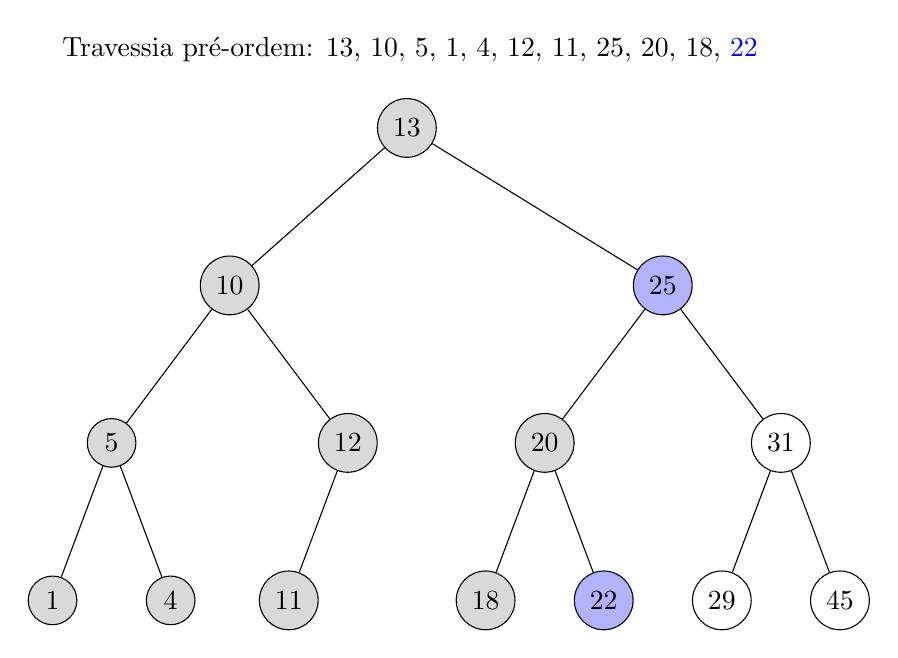
\begin{tikzpicture}

        \begin{scope}
            \node[anchor=west] (X) at (0, 6) { Travessia pré-ordem: 13, 10, 5, 1, 4, 12, 11, 25, 20, 18, \textcolor{blue}{22} };

            \node[circle,draw,fill=gray!30] (A) at (4.5, 5) { $13$ };
            \node[circle,draw,fill=gray!30] (B) at (2.25, 3) { $10$ };
            \node[circle,draw,fill=blue!30] (C) at (7.75, 3) { $25$ };
            \node[circle,draw,fill=gray!30] (D) at (0.75, 1) { $5$ };
            \node[circle,draw,fill=gray!30] (E) at (3.75, 1) { $12$ };
            \node[circle,draw,fill=gray!30] (F) at (6.25, 1) { $20$ };
            \node[circle,draw] (G) at (9.25, 1) { $31$ };
            \node[circle,draw,fill=gray!30] (H) at (0, -1) { $1$ };
            \node[circle,draw,fill=gray!30] (I) at (1.5, -1) { $4$ };
            \node[circle,draw,fill=gray!30] (J) at (3, -1) { $11$ };
            \node[circle,draw,fill=gray!30] (L) at (5.5, -1) { $18$ };
            \node[circle,draw,fill=blue!30] (M) at (7, -1) { $22$ };
            \node[circle,draw] (N) at (8.5, -1) { $29$ };
            \node[circle,draw] (O) at (10, -1) { $45$ };

            \draw (A) -- (B);
            \draw (A) -- (C);
            \draw (B) -- (D);
            \draw (B) -- (E);
            \draw (C) -- (F);
            \draw (C) -- (G);

            \draw (D) -- (H);
            \draw (D) -- (I);
            \draw (E) -- (J);
            \draw (F) -- (L);
            \draw (F) -- (M);
            \draw (G) -- (N);
            \draw (G) -- (O);
        \end{scope}
    \end{tikzpicture}

\end{frame}

\begin{frame}[fragile]{Exemplo de inserção em árvore binária de busca}

    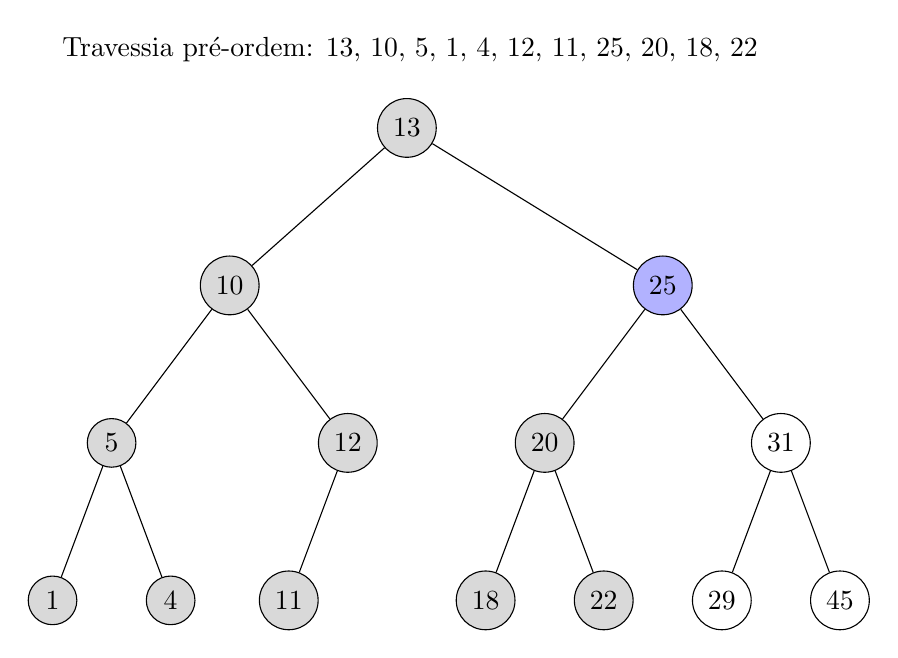
\begin{tikzpicture}

        \begin{scope}
            \node[anchor=west] (X) at (0, 6) { Travessia pré-ordem: 13, 10, 5, 1, 4, 12, 11, 25, 20, 18, 22 \textcolor{blue}{} };

            \node[circle,draw,fill=gray!30] (A) at (4.5, 5) { $13$ };
            \node[circle,draw,fill=gray!30] (B) at (2.25, 3) { $10$ };
            \node[circle,draw,fill=blue!30] (C) at (7.75, 3) { $25$ };
            \node[circle,draw,fill=gray!30] (D) at (0.75, 1) { $5$ };
            \node[circle,draw,fill=gray!30] (E) at (3.75, 1) { $12$ };
            \node[circle,draw,fill=gray!30] (F) at (6.25, 1) { $20$ };
            \node[circle,draw] (G) at (9.25, 1) { $31$ };
            \node[circle,draw,fill=gray!30] (H) at (0, -1) { $1$ };
            \node[circle,draw,fill=gray!30] (I) at (1.5, -1) { $4$ };
            \node[circle,draw,fill=gray!30] (J) at (3, -1) { $11$ };
            \node[circle,draw,fill=gray!30] (L) at (5.5, -1) { $18$ };
            \node[circle,draw,fill=gray!30] (M) at (7, -1) { $22$ };
            \node[circle,draw] (N) at (8.5, -1) { $29$ };
            \node[circle,draw] (O) at (10, -1) { $45$ };

            \draw (A) -- (B);
            \draw (A) -- (C);
            \draw (B) -- (D);
            \draw (B) -- (E);
            \draw (C) -- (F);
            \draw (C) -- (G);

            \draw (D) -- (H);
            \draw (D) -- (I);
            \draw (E) -- (J);
            \draw (F) -- (L);
            \draw (F) -- (M);
            \draw (G) -- (N);
            \draw (G) -- (O);
        \end{scope}
    \end{tikzpicture}

\end{frame}

\begin{frame}[fragile]{Exemplo de inserção em árvore binária de busca}

    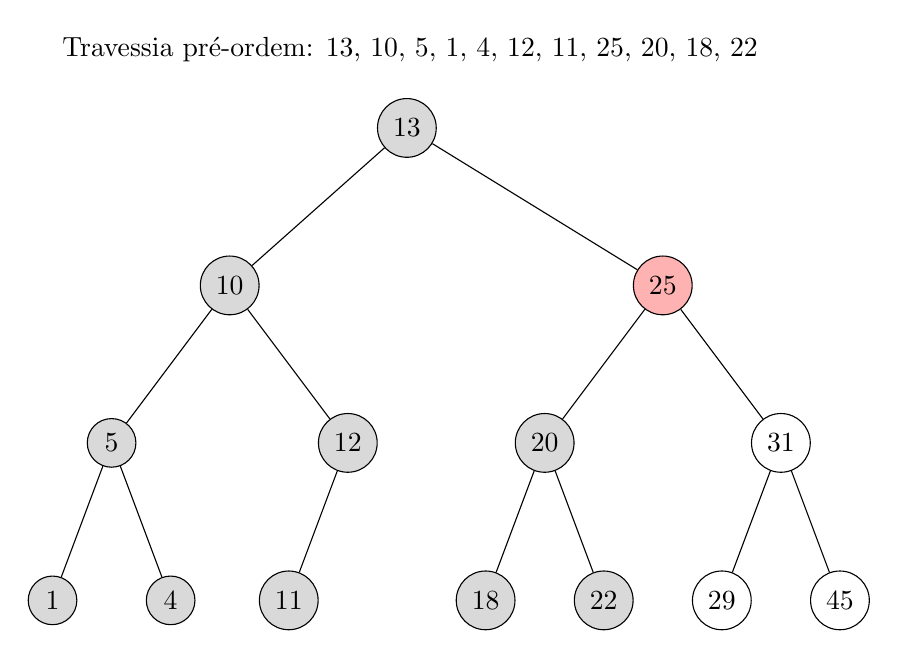
\begin{tikzpicture}

        \begin{scope}
            \node[anchor=west] (X) at (0, 6) { Travessia pré-ordem: 13, 10, 5, 1, 4, 12, 11, 25, 20, 18, 22 \textcolor{blue}{} };

            \node[circle,draw,fill=gray!30] (A) at (4.5, 5) { $13$ };
            \node[circle,draw,fill=gray!30] (B) at (2.25, 3) { $10$ };
            \node[circle,draw,fill=red!30] (C) at (7.75, 3) { $25$ };
            \node[circle,draw,fill=gray!30] (D) at (0.75, 1) { $5$ };
            \node[circle,draw,fill=gray!30] (E) at (3.75, 1) { $12$ };
            \node[circle,draw,fill=gray!30] (F) at (6.25, 1) { $20$ };
            \node[circle,draw] (G) at (9.25, 1) { $31$ };
            \node[circle,draw,fill=gray!30] (H) at (0, -1) { $1$ };
            \node[circle,draw,fill=gray!30] (I) at (1.5, -1) { $4$ };
            \node[circle,draw,fill=gray!30] (J) at (3, -1) { $11$ };
            \node[circle,draw,fill=gray!30] (L) at (5.5, -1) { $18$ };
            \node[circle,draw,fill=gray!30] (M) at (7, -1) { $22$ };
            \node[circle,draw] (N) at (8.5, -1) { $29$ };
            \node[circle,draw] (O) at (10, -1) { $45$ };

            \draw (A) -- (B);
            \draw (A) -- (C);
            \draw (B) -- (D);
            \draw (B) -- (E);
            \draw (C) -- (F);
            \draw (C) -- (G);

            \draw (D) -- (H);
            \draw (D) -- (I);
            \draw (E) -- (J);
            \draw (F) -- (L);
            \draw (F) -- (M);
            \draw (G) -- (N);
            \draw (G) -- (O);
        \end{scope}
    \end{tikzpicture}

\end{frame}

\begin{frame}[fragile]{Exemplo de inserção em árvore binária de busca}

    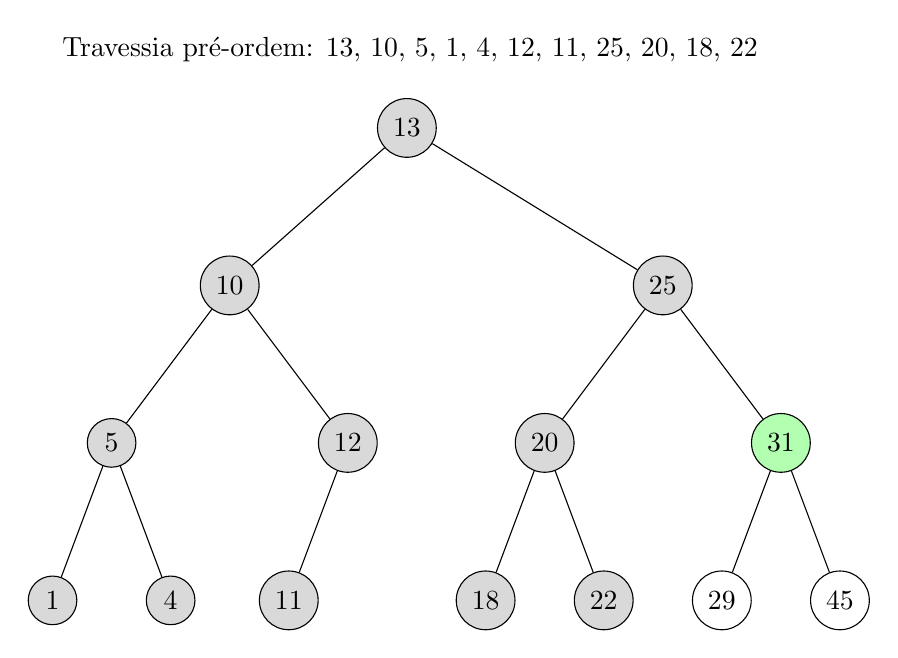
\begin{tikzpicture}

        \begin{scope}
            \node[anchor=west] (X) at (0, 6) { Travessia pré-ordem: 13, 10, 5, 1, 4, 12, 11, 25, 20, 18, 22 \textcolor{blue}{} };

            \node[circle,draw,fill=gray!30] (A) at (4.5, 5) { $13$ };
            \node[circle,draw,fill=gray!30] (B) at (2.25, 3) { $10$ };
            \node[circle,draw,fill=gray!30] (C) at (7.75, 3) { $25$ };
            \node[circle,draw,fill=gray!30] (D) at (0.75, 1) { $5$ };
            \node[circle,draw,fill=gray!30] (E) at (3.75, 1) { $12$ };
            \node[circle,draw,fill=gray!30] (F) at (6.25, 1) { $20$ };
            \node[circle,draw,fill=green!30] (G) at (9.25, 1) { $31$ };
            \node[circle,draw,fill=gray!30] (H) at (0, -1) { $1$ };
            \node[circle,draw,fill=gray!30] (I) at (1.5, -1) { $4$ };
            \node[circle,draw,fill=gray!30] (J) at (3, -1) { $11$ };
            \node[circle,draw,fill=gray!30] (L) at (5.5, -1) { $18$ };
            \node[circle,draw,fill=gray!30] (M) at (7, -1) { $22$ };
            \node[circle,draw] (N) at (8.5, -1) { $29$ };
            \node[circle,draw] (O) at (10, -1) { $45$ };

            \draw (A) -- (B);
            \draw (A) -- (C);
            \draw (B) -- (D);
            \draw (B) -- (E);
            \draw (C) -- (F);
            \draw (C) -- (G);

            \draw (D) -- (H);
            \draw (D) -- (I);
            \draw (E) -- (J);
            \draw (F) -- (L);
            \draw (F) -- (M);
            \draw (G) -- (N);
            \draw (G) -- (O);
        \end{scope}
    \end{tikzpicture}

\end{frame}

\begin{frame}[fragile]{Exemplo de inserção em árvore binária de busca}

    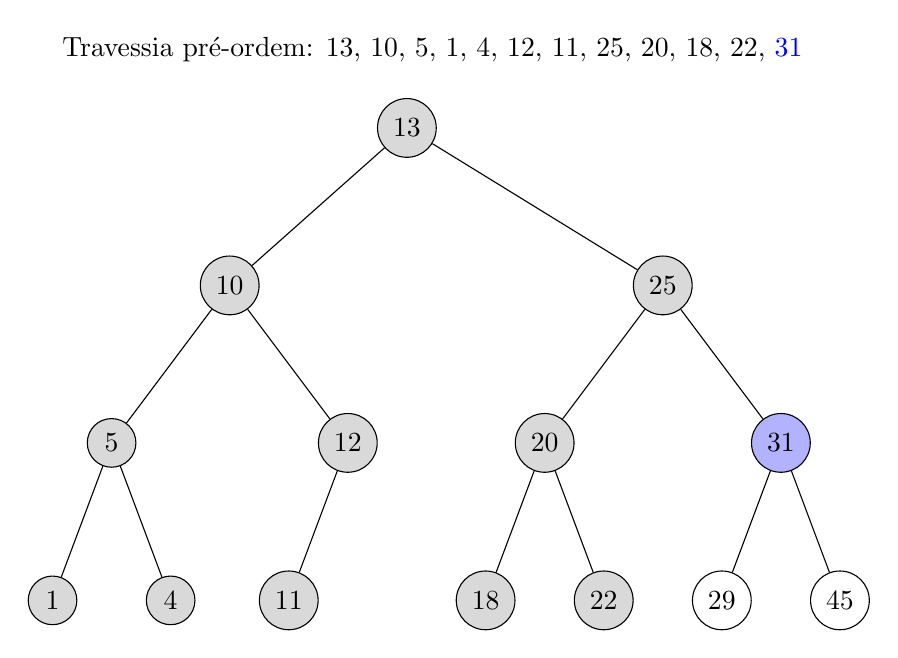
\begin{tikzpicture}

        \begin{scope}
            \node[anchor=west] (X) at (0, 6) { Travessia pré-ordem: 13, 10, 5, 1, 4, 12, 11, 25, 20, 18, 22, \textcolor{blue}{31} };

            \node[circle,draw,fill=gray!30] (A) at (4.5, 5) { $13$ };
            \node[circle,draw,fill=gray!30] (B) at (2.25, 3) { $10$ };
            \node[circle,draw,fill=gray!30] (C) at (7.75, 3) { $25$ };
            \node[circle,draw,fill=gray!30] (D) at (0.75, 1) { $5$ };
            \node[circle,draw,fill=gray!30] (E) at (3.75, 1) { $12$ };
            \node[circle,draw,fill=gray!30] (F) at (6.25, 1) { $20$ };
            \node[circle,draw,fill=blue!30] (G) at (9.25, 1) { $31$ };
            \node[circle,draw,fill=gray!30] (H) at (0, -1) { $1$ };
            \node[circle,draw,fill=gray!30] (I) at (1.5, -1) { $4$ };
            \node[circle,draw,fill=gray!30] (J) at (3, -1) { $11$ };
            \node[circle,draw,fill=gray!30] (L) at (5.5, -1) { $18$ };
            \node[circle,draw,fill=gray!30] (M) at (7, -1) { $22$ };
            \node[circle,draw] (N) at (8.5, -1) { $29$ };
            \node[circle,draw] (O) at (10, -1) { $45$ };

            \draw (A) -- (B);
            \draw (A) -- (C);
            \draw (B) -- (D);
            \draw (B) -- (E);
            \draw (C) -- (F);
            \draw (C) -- (G);

            \draw (D) -- (H);
            \draw (D) -- (I);
            \draw (E) -- (J);
            \draw (F) -- (L);
            \draw (F) -- (M);
            \draw (G) -- (N);
            \draw (G) -- (O);
        \end{scope}
    \end{tikzpicture}

\end{frame}

\begin{frame}[fragile]{Exemplo de inserção em árvore binária de busca}

    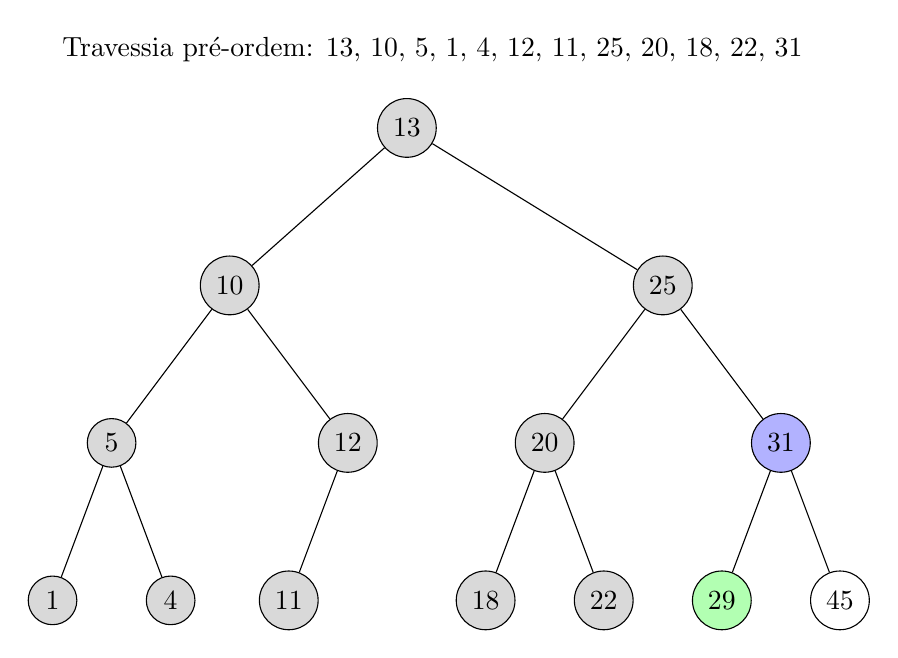
\begin{tikzpicture}

        \begin{scope}
            \node[anchor=west] (X) at (0, 6) { Travessia pré-ordem: 13, 10, 5, 1, 4, 12, 11, 25, 20, 18, 22, 31 \textcolor{blue}{} };

            \node[circle,draw,fill=gray!30] (A) at (4.5, 5) { $13$ };
            \node[circle,draw,fill=gray!30] (B) at (2.25, 3) { $10$ };
            \node[circle,draw,fill=gray!30] (C) at (7.75, 3) { $25$ };
            \node[circle,draw,fill=gray!30] (D) at (0.75, 1) { $5$ };
            \node[circle,draw,fill=gray!30] (E) at (3.75, 1) { $12$ };
            \node[circle,draw,fill=gray!30] (F) at (6.25, 1) { $20$ };
            \node[circle,draw,fill=blue!30] (G) at (9.25, 1) { $31$ };
            \node[circle,draw,fill=gray!30] (H) at (0, -1) { $1$ };
            \node[circle,draw,fill=gray!30] (I) at (1.5, -1) { $4$ };
            \node[circle,draw,fill=gray!30] (J) at (3, -1) { $11$ };
            \node[circle,draw,fill=gray!30] (L) at (5.5, -1) { $18$ };
            \node[circle,draw,fill=gray!30] (M) at (7, -1) { $22$ };
            \node[circle,draw,fill=green!30] (N) at (8.5, -1) { $29$ };
            \node[circle,draw] (O) at (10, -1) { $45$ };

            \draw (A) -- (B);
            \draw (A) -- (C);
            \draw (B) -- (D);
            \draw (B) -- (E);
            \draw (C) -- (F);
            \draw (C) -- (G);

            \draw (D) -- (H);
            \draw (D) -- (I);
            \draw (E) -- (J);
            \draw (F) -- (L);
            \draw (F) -- (M);
            \draw (G) -- (N);
            \draw (G) -- (O);
        \end{scope}
    \end{tikzpicture}

\end{frame}

\begin{frame}[fragile]{Exemplo de inserção em árvore binária de busca}

    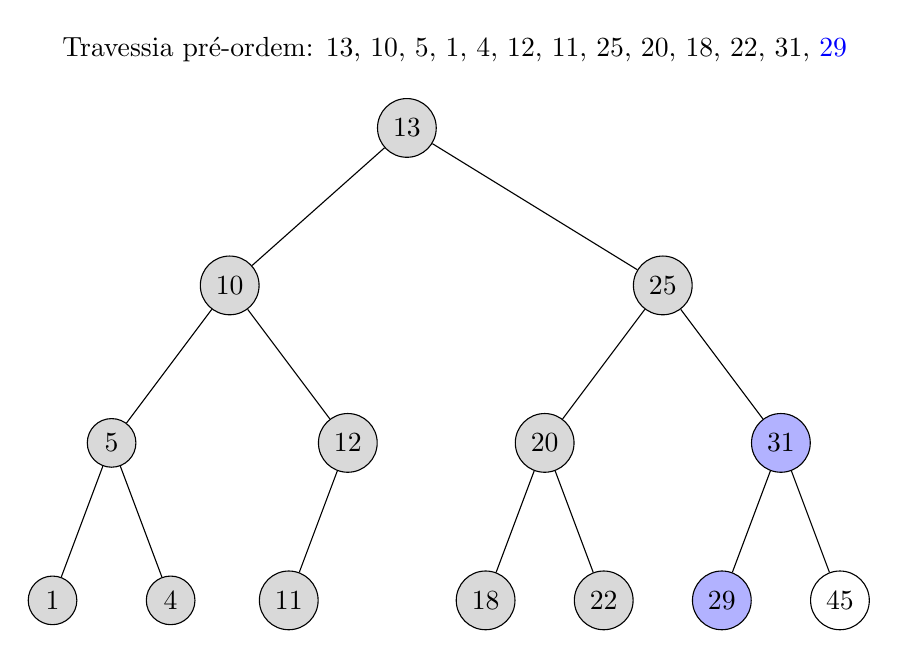
\begin{tikzpicture}

        \begin{scope}
            \node[anchor=west] (X) at (0, 6) { Travessia pré-ordem: 13, 10, 5, 1, 4, 12, 11, 25, 20, 18, 22, 31, \textcolor{blue}{29} };

            \node[circle,draw,fill=gray!30] (A) at (4.5, 5) { $13$ };
            \node[circle,draw,fill=gray!30] (B) at (2.25, 3) { $10$ };
            \node[circle,draw,fill=gray!30] (C) at (7.75, 3) { $25$ };
            \node[circle,draw,fill=gray!30] (D) at (0.75, 1) { $5$ };
            \node[circle,draw,fill=gray!30] (E) at (3.75, 1) { $12$ };
            \node[circle,draw,fill=gray!30] (F) at (6.25, 1) { $20$ };
            \node[circle,draw,fill=blue!30] (G) at (9.25, 1) { $31$ };
            \node[circle,draw,fill=gray!30] (H) at (0, -1) { $1$ };
            \node[circle,draw,fill=gray!30] (I) at (1.5, -1) { $4$ };
            \node[circle,draw,fill=gray!30] (J) at (3, -1) { $11$ };
            \node[circle,draw,fill=gray!30] (L) at (5.5, -1) { $18$ };
            \node[circle,draw,fill=gray!30] (M) at (7, -1) { $22$ };
            \node[circle,draw,fill=blue!30] (N) at (8.5, -1) { $29$ };
            \node[circle,draw] (O) at (10, -1) { $45$ };

            \draw (A) -- (B);
            \draw (A) -- (C);
            \draw (B) -- (D);
            \draw (B) -- (E);
            \draw (C) -- (F);
            \draw (C) -- (G);

            \draw (D) -- (H);
            \draw (D) -- (I);
            \draw (E) -- (J);
            \draw (F) -- (L);
            \draw (F) -- (M);
            \draw (G) -- (N);
            \draw (G) -- (O);
        \end{scope}
    \end{tikzpicture}

\end{frame}

\begin{frame}[fragile]{Exemplo de inserção em árvore binária de busca}

    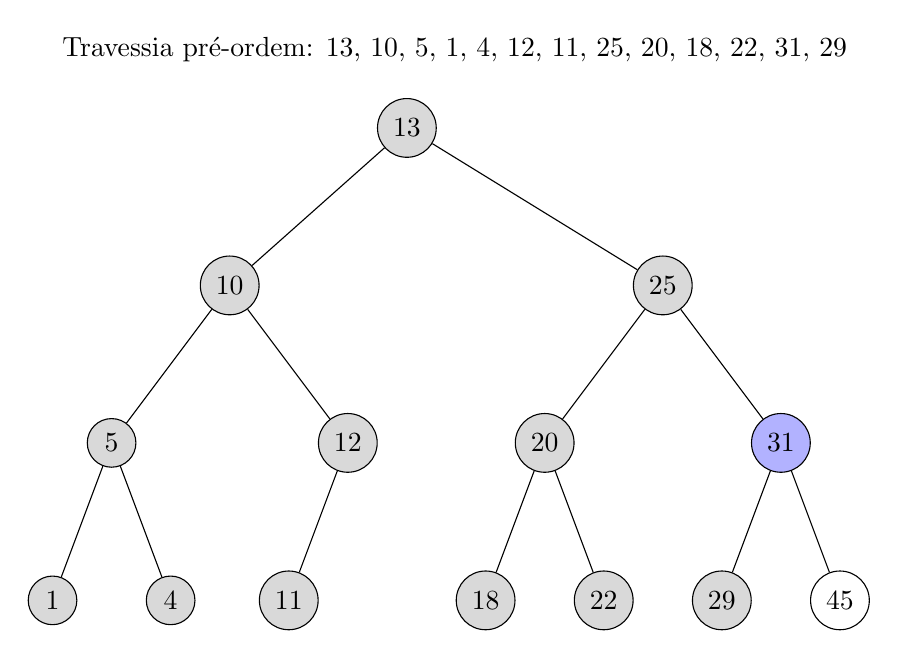
\begin{tikzpicture}

        \begin{scope}
            \node[anchor=west] (X) at (0, 6) { Travessia pré-ordem: 13, 10, 5, 1, 4, 12, 11, 25, 20, 18, 22, 31, 29 \textcolor{blue}{} };

            \node[circle,draw,fill=gray!30] (A) at (4.5, 5) { $13$ };
            \node[circle,draw,fill=gray!30] (B) at (2.25, 3) { $10$ };
            \node[circle,draw,fill=gray!30] (C) at (7.75, 3) { $25$ };
            \node[circle,draw,fill=gray!30] (D) at (0.75, 1) { $5$ };
            \node[circle,draw,fill=gray!30] (E) at (3.75, 1) { $12$ };
            \node[circle,draw,fill=gray!30] (F) at (6.25, 1) { $20$ };
            \node[circle,draw,fill=blue!30] (G) at (9.25, 1) { $31$ };
            \node[circle,draw,fill=gray!30] (H) at (0, -1) { $1$ };
            \node[circle,draw,fill=gray!30] (I) at (1.5, -1) { $4$ };
            \node[circle,draw,fill=gray!30] (J) at (3, -1) { $11$ };
            \node[circle,draw,fill=gray!30] (L) at (5.5, -1) { $18$ };
            \node[circle,draw,fill=gray!30] (M) at (7, -1) { $22$ };
            \node[circle,draw,fill=gray!30] (N) at (8.5, -1) { $29$ };
            \node[circle,draw] (O) at (10, -1) { $45$ };

            \draw (A) -- (B);
            \draw (A) -- (C);
            \draw (B) -- (D);
            \draw (B) -- (E);
            \draw (C) -- (F);
            \draw (C) -- (G);

            \draw (D) -- (H);
            \draw (D) -- (I);
            \draw (E) -- (J);
            \draw (F) -- (L);
            \draw (F) -- (M);
            \draw (G) -- (N);
            \draw (G) -- (O);
        \end{scope}
    \end{tikzpicture}

\end{frame}

\begin{frame}[fragile]{Exemplo de inserção em árvore binária de busca}

    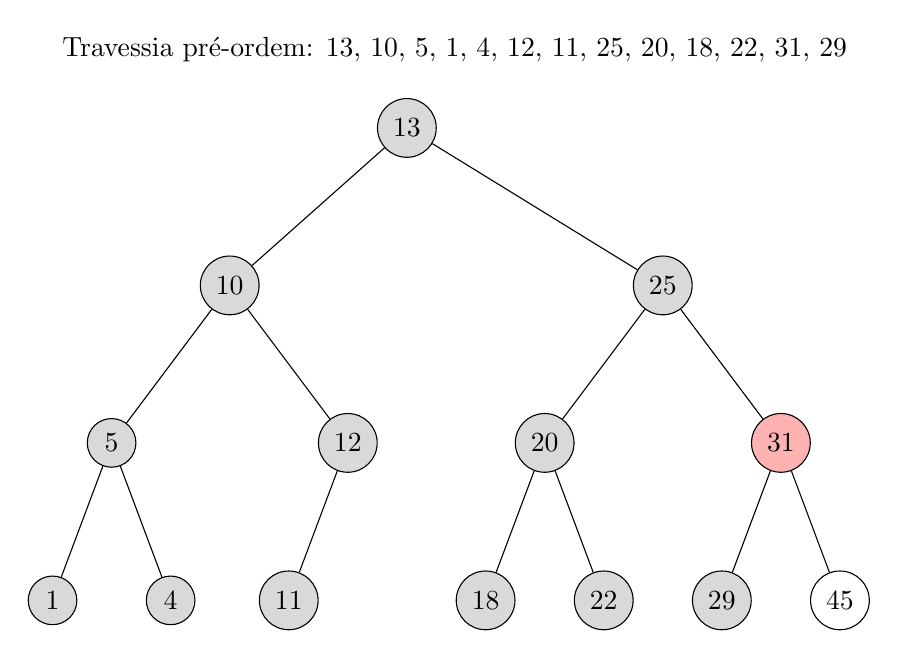
\begin{tikzpicture}

        \begin{scope}
            \node[anchor=west] (X) at (0, 6) { Travessia pré-ordem: 13, 10, 5, 1, 4, 12, 11, 25, 20, 18, 22, 31, 29 \textcolor{blue}{} };

            \node[circle,draw,fill=gray!30] (A) at (4.5, 5) { $13$ };
            \node[circle,draw,fill=gray!30] (B) at (2.25, 3) { $10$ };
            \node[circle,draw,fill=gray!30] (C) at (7.75, 3) { $25$ };
            \node[circle,draw,fill=gray!30] (D) at (0.75, 1) { $5$ };
            \node[circle,draw,fill=gray!30] (E) at (3.75, 1) { $12$ };
            \node[circle,draw,fill=gray!30] (F) at (6.25, 1) { $20$ };
            \node[circle,draw,fill=red!30] (G) at (9.25, 1) { $31$ };
            \node[circle,draw,fill=gray!30] (H) at (0, -1) { $1$ };
            \node[circle,draw,fill=gray!30] (I) at (1.5, -1) { $4$ };
            \node[circle,draw,fill=gray!30] (J) at (3, -1) { $11$ };
            \node[circle,draw,fill=gray!30] (L) at (5.5, -1) { $18$ };
            \node[circle,draw,fill=gray!30] (M) at (7, -1) { $22$ };
            \node[circle,draw,fill=gray!30] (N) at (8.5, -1) { $29$ };
            \node[circle,draw] (O) at (10, -1) { $45$ };

            \draw (A) -- (B);
            \draw (A) -- (C);
            \draw (B) -- (D);
            \draw (B) -- (E);
            \draw (C) -- (F);
            \draw (C) -- (G);

            \draw (D) -- (H);
            \draw (D) -- (I);
            \draw (E) -- (J);
            \draw (F) -- (L);
            \draw (F) -- (M);
            \draw (G) -- (N);
            \draw (G) -- (O);
        \end{scope}
    \end{tikzpicture}

\end{frame}

\begin{frame}[fragile]{Exemplo de inserção em árvore binária de busca}

    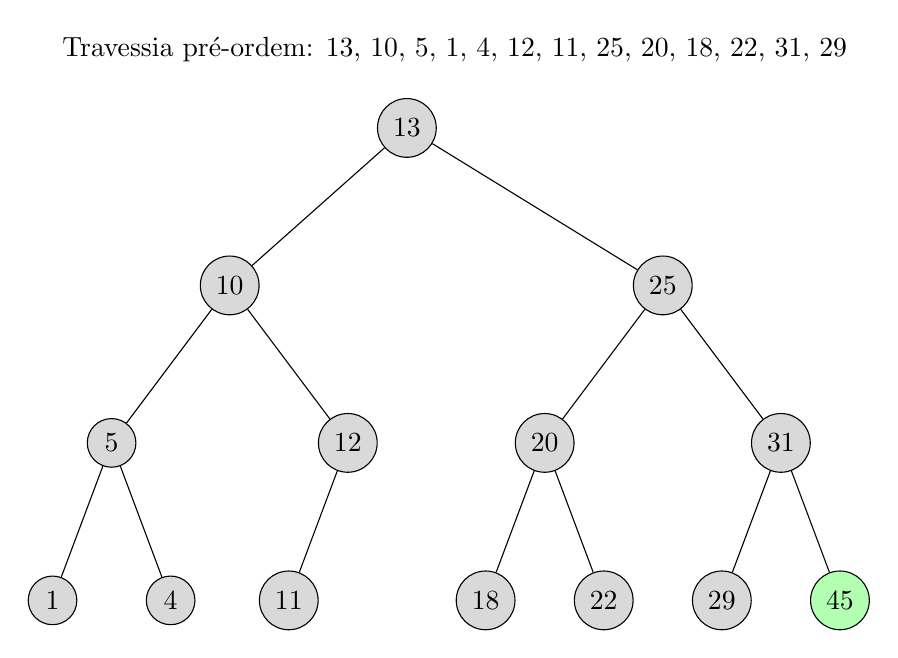
\begin{tikzpicture}

        \begin{scope}
            \node[anchor=west] (X) at (0, 6) { Travessia pré-ordem: 13, 10, 5, 1, 4, 12, 11, 25, 20, 18, 22, 31, 29 \textcolor{blue}{} };

            \node[circle,draw,fill=gray!30] (A) at (4.5, 5) { $13$ };
            \node[circle,draw,fill=gray!30] (B) at (2.25, 3) { $10$ };
            \node[circle,draw,fill=gray!30] (C) at (7.75, 3) { $25$ };
            \node[circle,draw,fill=gray!30] (D) at (0.75, 1) { $5$ };
            \node[circle,draw,fill=gray!30] (E) at (3.75, 1) { $12$ };
            \node[circle,draw,fill=gray!30] (F) at (6.25, 1) { $20$ };
            \node[circle,draw,fill=gray!30] (G) at (9.25, 1) { $31$ };
            \node[circle,draw,fill=gray!30] (H) at (0, -1) { $1$ };
            \node[circle,draw,fill=gray!30] (I) at (1.5, -1) { $4$ };
            \node[circle,draw,fill=gray!30] (J) at (3, -1) { $11$ };
            \node[circle,draw,fill=gray!30] (L) at (5.5, -1) { $18$ };
            \node[circle,draw,fill=gray!30] (M) at (7, -1) { $22$ };
            \node[circle,draw,fill=gray!30] (N) at (8.5, -1) { $29$ };
            \node[circle,draw,fill=green!30] (O) at (10, -1) { $45$ };

            \draw (A) -- (B);
            \draw (A) -- (C);
            \draw (B) -- (D);
            \draw (B) -- (E);
            \draw (C) -- (F);
            \draw (C) -- (G);

            \draw (D) -- (H);
            \draw (D) -- (I);
            \draw (E) -- (J);
            \draw (F) -- (L);
            \draw (F) -- (M);
            \draw (G) -- (N);
            \draw (G) -- (O);
        \end{scope}
    \end{tikzpicture}

\end{frame}

\begin{frame}[fragile]{Exemplo de inserção em árvore binária de busca}

    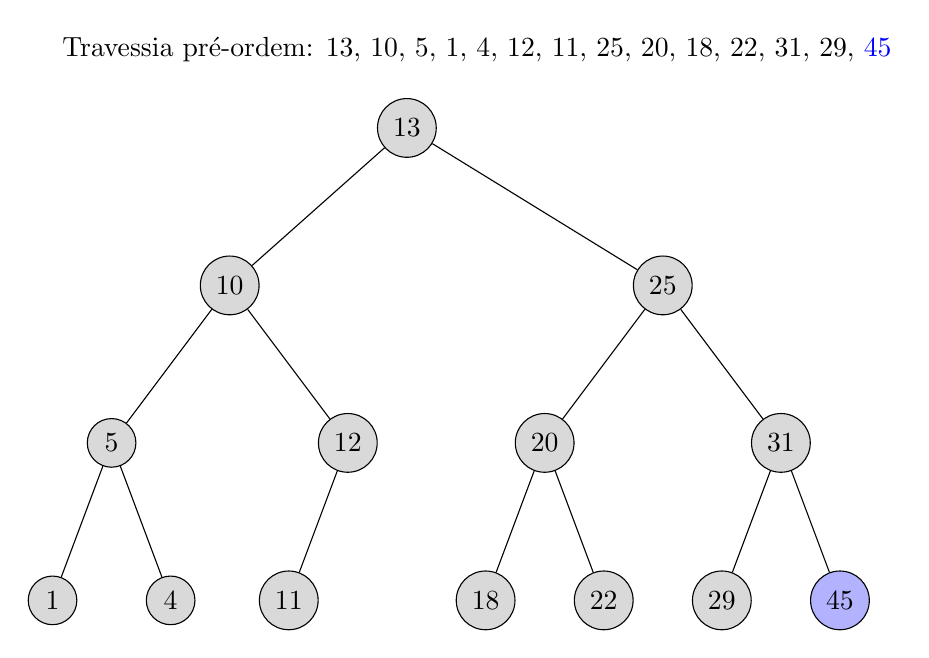
\begin{tikzpicture}

        \begin{scope}
            \node[anchor=west] (X) at (0, 6) { Travessia pré-ordem: 13, 10, 5, 1, 4, 12, 11, 25, 20, 18, 22, 31, 29, \textcolor{blue}{45} };

            \node[circle,draw,fill=gray!30] (A) at (4.5, 5) { $13$ };
            \node[circle,draw,fill=gray!30] (B) at (2.25, 3) { $10$ };
            \node[circle,draw,fill=gray!30] (C) at (7.75, 3) { $25$ };
            \node[circle,draw,fill=gray!30] (D) at (0.75, 1) { $5$ };
            \node[circle,draw,fill=gray!30] (E) at (3.75, 1) { $12$ };
            \node[circle,draw,fill=gray!30] (F) at (6.25, 1) { $20$ };
            \node[circle,draw,fill=gray!30] (G) at (9.25, 1) { $31$ };
            \node[circle,draw,fill=gray!30] (H) at (0, -1) { $1$ };
            \node[circle,draw,fill=gray!30] (I) at (1.5, -1) { $4$ };
            \node[circle,draw,fill=gray!30] (J) at (3, -1) { $11$ };
            \node[circle,draw,fill=gray!30] (L) at (5.5, -1) { $18$ };
            \node[circle,draw,fill=gray!30] (M) at (7, -1) { $22$ };
            \node[circle,draw,fill=gray!30] (N) at (8.5, -1) { $29$ };
            \node[circle,draw,fill=blue!30] (O) at (10, -1) { $45$ };

            \draw (A) -- (B);
            \draw (A) -- (C);
            \draw (B) -- (D);
            \draw (B) -- (E);
            \draw (C) -- (F);
            \draw (C) -- (G);

            \draw (D) -- (H);
            \draw (D) -- (I);
            \draw (E) -- (J);
            \draw (F) -- (L);
            \draw (F) -- (M);
            \draw (G) -- (N);
            \draw (G) -- (O);
        \end{scope}
    \end{tikzpicture}

\end{frame}

\begin{frame}[fragile]{Exemplo de inserção em árvore binária de busca}

    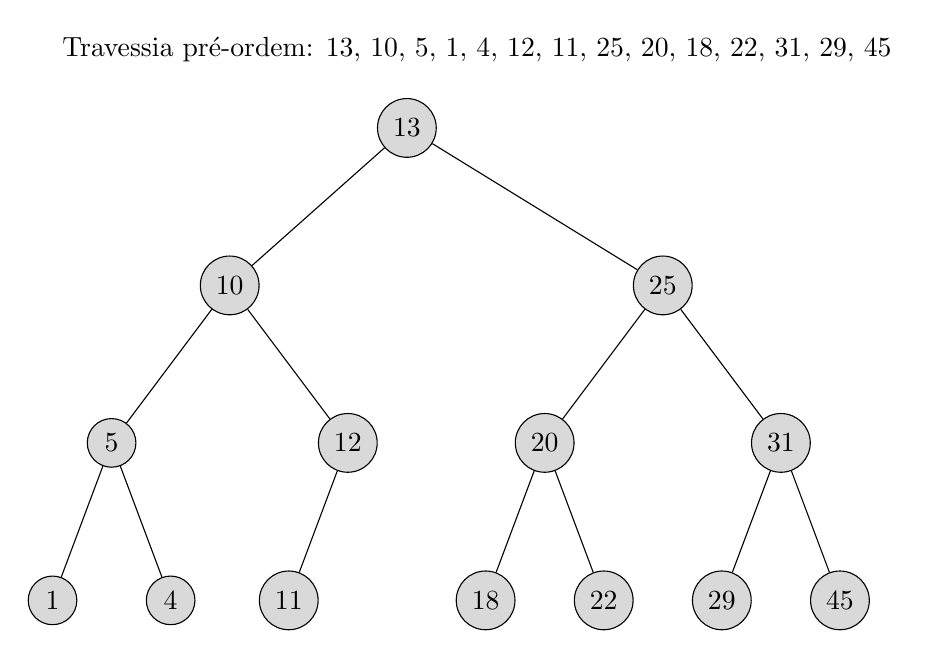
\begin{tikzpicture}

        \begin{scope}
            \node[anchor=west] (X) at (0, 6) { Travessia pré-ordem: 13, 10, 5, 1, 4, 12, 11, 25, 20, 18, 22, 31, 29, 45 \textcolor{blue}{} };

            \node[circle,draw,fill=gray!30] (A) at (4.5, 5) { $13$ };
            \node[circle,draw,fill=gray!30] (B) at (2.25, 3) { $10$ };
            \node[circle,draw,fill=gray!30] (C) at (7.75, 3) { $25$ };
            \node[circle,draw,fill=gray!30] (D) at (0.75, 1) { $5$ };
            \node[circle,draw,fill=gray!30] (E) at (3.75, 1) { $12$ };
            \node[circle,draw,fill=gray!30] (F) at (6.25, 1) { $20$ };
            \node[circle,draw,fill=gray!30] (G) at (9.25, 1) { $31$ };
            \node[circle,draw,fill=gray!30] (H) at (0, -1) { $1$ };
            \node[circle,draw,fill=gray!30] (I) at (1.5, -1) { $4$ };
            \node[circle,draw,fill=gray!30] (J) at (3, -1) { $11$ };
            \node[circle,draw,fill=gray!30] (L) at (5.5, -1) { $18$ };
            \node[circle,draw,fill=gray!30] (M) at (7, -1) { $22$ };
            \node[circle,draw,fill=gray!30] (N) at (8.5, -1) { $29$ };
            \node[circle,draw,fill=gray!30] (O) at (10, -1) { $45$ };

            \draw (A) -- (B);
            \draw (A) -- (C);
            \draw (B) -- (D);
            \draw (B) -- (E);
            \draw (C) -- (F);
            \draw (C) -- (G);

            \draw (D) -- (H);
            \draw (D) -- (I);
            \draw (E) -- (J);
            \draw (F) -- (L);
            \draw (F) -- (M);
            \draw (G) -- (N);
            \draw (G) -- (O);
        \end{scope}
    \end{tikzpicture}

\end{frame}

\begin{frame}[fragile]{Implementação das travessias notáveis em C++}
    \inputsnippet{cpp}{1}{21}{traversal.cpp}
\end{frame}

\begin{frame}[fragile]{Implementação das travessias notáveis em C++}
    \inputsnippet{cpp}{22}{42}{traversal.cpp}
\end{frame}

\begin{frame}[fragile]{Reconstrução de árvores binárias a partir de travessias}

    \begin{itemize}
        \item Das três  travessias notáveis de uma árvore binária de busca, duas permitem
            a reconstrução da árvore original: a pré-ordem e a pós-ordem

        \item Veja que a travessia em-ordem não garante a unicidade da árvore: as árvores 
            abaixo tem a mesma travessia em-ordem, e são distintas
    \end{itemize}

    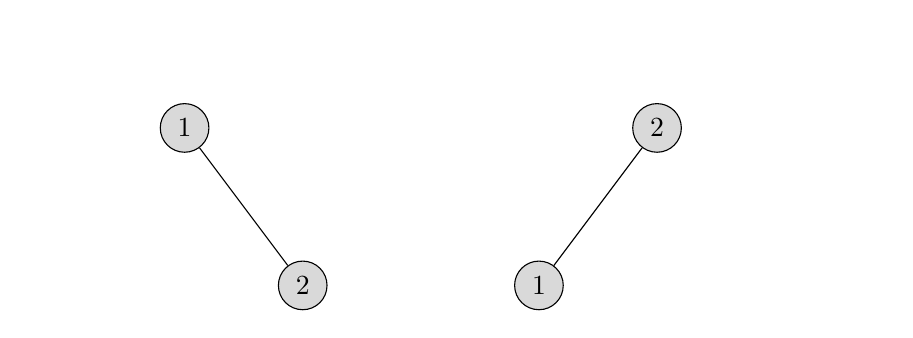
\begin{tikzpicture}

        \begin{scope}
            \node[opacity=0,anchor=west] (X) at (0, 6) { Travessia pré-ordem: 13, 10, 5, 1, 4, 12, 11, 25, 20, 18, 22, 31, 29, 45 \textcolor{blue}{} };

            \node[circle,draw,fill=gray!30] (A) at (2, 5) { $1$ };
            \node[circle,draw,fill=gray!30] (B) at (3.5, 3) { $2$ };


            \node[circle,draw,fill=gray!30] (C) at (8, 5) { $2$ };
            \node[circle,draw,fill=gray!30] (D) at (6.5, 3) { $1$ };

            \draw (A) -- (B);
            \draw (D) -- (C);
       \end{scope}
    \end{tikzpicture}

\end{frame}

\begin{frame}[fragile]{Reconstrução de árvores binárias a partir de travessias}

    \begin{itemize}
        \item Para uma árvore binária qualquer, um par de travessias, exceto o par
            pré-ordem/pós-ordem, garante a unicidade de árvore

        \item Em outras palavras, a travessia em em-ordem, mais um das outras duas travessias,
            garante a unicidade de árvore

        \item Isto porque a travessia em-ordem estabelece a ordem relativa dos elementos, a qual
            fica subentendida numa árvore binária de busca

        \item Por este motivo a árvore binária de busca pode ser reconstruída usando apenas a
            pré-ordem ou a pós-ordem

        \item Para tal, basta inserir os elementos na ordem listada na pré-ordem (ou em ordem
            reversa, na pós-ordem) e usar a ordenação estabelecida na em-ordem para posicionar
            os elementos na inserção
    \end{itemize}

\end{frame}

\begin{frame}[fragile]{Exemplo de construção: pré-ordem e em-ordem}

    \begin{figure}
        \centering
        \begin{tikzpicture}
            \begin{scope}
                \node[anchor=west] (X) at (1, 6) { Travessia pré-ordem: A, B, C, D, E, F };
                \node[anchor=west] (X) at (1, 5.5) { Travessia em-ordem: B, C, A, E, D, F };

                \node[opacity=0,circle,draw,fill=gray!30] (A) at (4, 4.5) { A };
                \node[opacity=0,circle,draw,fill=gray!30] (B) at (2, 3) { B };
                \node[opacity=0,circle,draw,fill=gray!30] (C) at (3, 0.5) { C };
                \node[opacity=0,circle,draw,fill=gray!30] (D) at (6, 3) { D };
                \node[opacity=0,circle,draw,fill=gray!30] (E) at (5, 0.5) { E };
                \node[opacity=0,circle,draw,fill=gray!30] (F) at (7, 0.5) { F };

%                \draw (A) -- (B);
%                \draw (A) -- (D);
%                \draw (B) -- (C);
%                \draw (D) -- (E);
%                \draw (D) -- (F);
           \end{scope}
        \end{tikzpicture}
    \end{figure}
\end{frame}

\begin{frame}[fragile]{Exemplo de construção: pré-ordem e em-ordem}

    \begin{figure}
        \centering
        \begin{tikzpicture}
            \begin{scope}
                \node[anchor=west] (X) at (1, 6) { Travessia pré-ordem: \textcolor{blue}{A}, B, C, D, E, F };
                \node[anchor=west] (X) at (1, 5.5) { Travessia em-ordem: B, C, A, E, D, F };

                \node[opacity=0,circle,draw,fill=gray!30] (A) at (4, 4.5) { A };
                \node[opacity=0,circle,draw,fill=gray!30] (B) at (2, 3) { B };
                \node[opacity=0,circle,draw,fill=gray!30] (C) at (3, 0.5) { C };
                \node[opacity=0,circle,draw,fill=gray!30] (D) at (6, 3) { D };
                \node[opacity=0,circle,draw,fill=gray!30] (E) at (5, 0.5) { E };
                \node[opacity=0,circle,draw,fill=gray!30] (F) at (7, 0.5) { F };

%                \draw (A) -- (B);
%                \draw (A) -- (D);
%                \draw (B) -- (C);
%                \draw (D) -- (E);
%                \draw (D) -- (F);
           \end{scope}
        \end{tikzpicture}
    \end{figure}
\end{frame}

\begin{frame}[fragile]{Exemplo de construção: pré-ordem e em-ordem}

    \begin{figure}
        \centering
        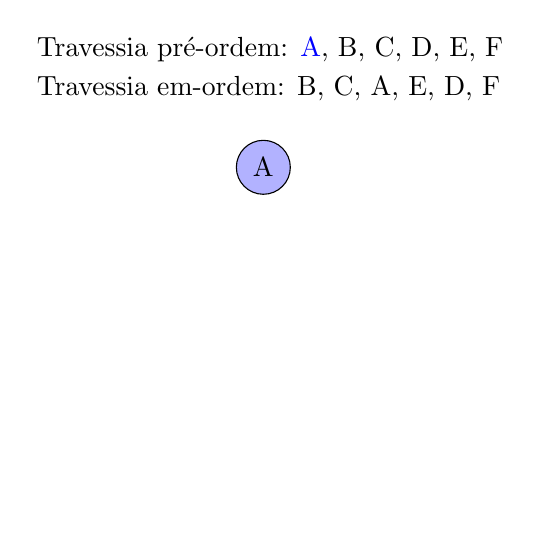
\begin{tikzpicture}
            \begin{scope}
                \node[anchor=west] (X) at (1, 6) { Travessia pré-ordem: \textcolor{blue}{A}, B, C, D, E, F };
                \node[anchor=west] (X) at (1, 5.5) { Travessia em-ordem: B, C, A, E, D, F };

                \node[circle,draw,fill=blue!30] (A) at (4, 4.5) { A };
                \node[opacity=0,circle,draw,fill=gray!30] (B) at (2, 3) { B };
                \node[opacity=0,circle,draw,fill=gray!30] (C) at (3, 0.5) { C };
                \node[opacity=0,circle,draw,fill=gray!30] (D) at (6, 3) { D };
                \node[opacity=0,circle,draw,fill=gray!30] (E) at (5, 0.5) { E };
                \node[opacity=0,circle,draw,fill=gray!30] (F) at (7, 0.5) { F };

%                \draw (A) -- (B);
%                \draw (A) -- (D);
%                \draw (B) -- (C);
%                \draw (D) -- (E);
%                \draw (D) -- (F);
           \end{scope}
        \end{tikzpicture}
    \end{figure}
\end{frame}

\begin{frame}[fragile]{Exemplo de construção: pré-ordem e em-ordem}

    \begin{figure}
        \centering
        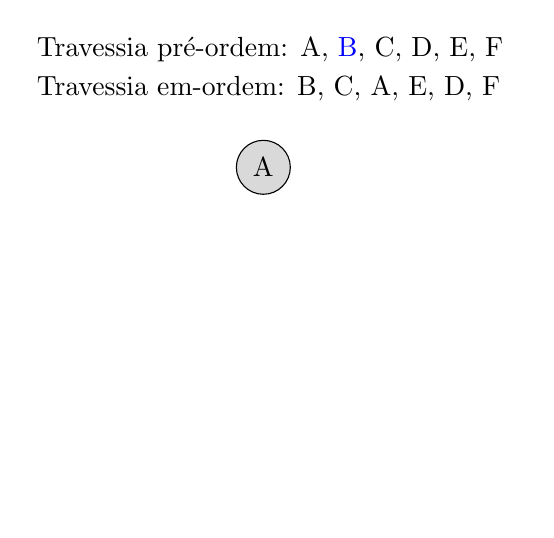
\begin{tikzpicture}
            \begin{scope}
                \node[anchor=west] (X) at (1, 6) { Travessia pré-ordem: A, \textcolor{blue}{B}, C, D, E, F };
                \node[anchor=west] (X) at (1, 5.5) { Travessia em-ordem: B, C, A, E, D, F };

                \node[circle,draw,fill=gray!30] (A) at (4, 4.5) { A };
                \node[opacity=0,circle,draw,fill=gray!30] (B) at (2, 3) { B };
                \node[opacity=0,circle,draw,fill=gray!30] (C) at (3, 0.5) { C };
                \node[opacity=0,circle,draw,fill=gray!30] (D) at (6, 3) { D };
                \node[opacity=0,circle,draw,fill=gray!30] (E) at (5, 0.5) { E };
                \node[opacity=0,circle,draw,fill=gray!30] (F) at (7, 0.5) { F };

%                \draw (A) -- (B);
%                \draw (A) -- (D);
%                \draw (B) -- (C);
%                \draw (D) -- (E);
%                \draw (D) -- (F);
           \end{scope}
        \end{tikzpicture}
    \end{figure}
\end{frame}

\begin{frame}[fragile]{Exemplo de construção: pré-ordem e em-ordem}

    \begin{figure}
        \centering
        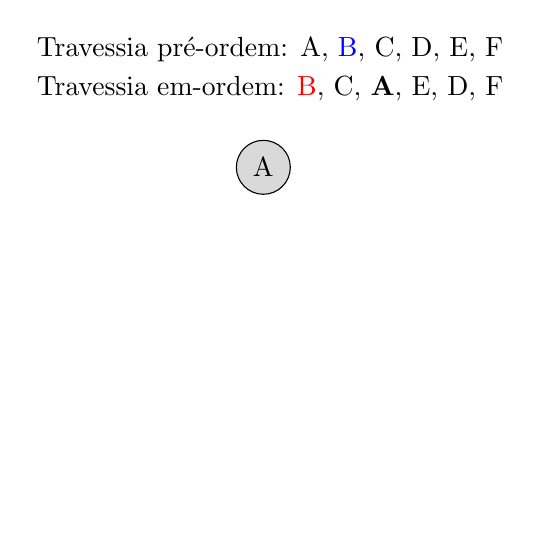
\begin{tikzpicture}
            \begin{scope}
                \node[anchor=west] (X) at (1, 6) { Travessia pré-ordem: A, \textcolor{blue}{B}, C, D, E, F };
                \node[anchor=west] (X) at (1, 5.5) { Travessia em-ordem: \textcolor{red}{B}, C, \textbf{A}, E, D, F };

                \node[circle,draw,fill=gray!30] (A) at (4, 4.5) { A };
                \node[opacity=0,circle,draw,fill=gray!30] (B) at (2, 3) { B };
                \node[opacity=0,circle,draw,fill=gray!30] (C) at (3, 0.5) { C };
                \node[opacity=0,circle,draw,fill=gray!30] (D) at (6, 3) { D };
                \node[opacity=0,circle,draw,fill=gray!30] (E) at (5, 0.5) { E };
                \node[opacity=0,circle,draw,fill=gray!30] (F) at (7, 0.5) { F };

%                \draw (A) -- (B);
%                \draw (A) -- (D);
%                \draw (B) -- (C);
%                \draw (D) -- (E);
%                \draw (D) -- (F);
           \end{scope}
        \end{tikzpicture}
    \end{figure}
\end{frame}

\begin{frame}[fragile]{Exemplo de construção: pré-ordem e em-ordem}

    \begin{figure}
        \centering
        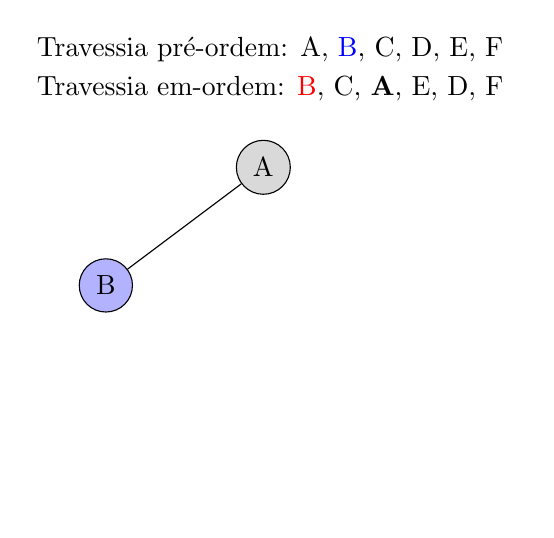
\begin{tikzpicture}
            \begin{scope}
                \node[anchor=west] (X) at (1, 6) { Travessia pré-ordem: A, \textcolor{blue}{B}, C, D, E, F };
                \node[anchor=west] (X) at (1, 5.5) { Travessia em-ordem: \textcolor{red}{B}, C, \textbf{A}, E, D, F };

                \node[circle,draw,fill=gray!30] (A) at (4, 4.5) { A };
                \node[circle,draw,fill=blue!30] (B) at (2, 3) { B };
                \node[opacity=0,circle,draw,fill=gray!30] (C) at (3, 0.5) { C };
                \node[opacity=0,circle,draw,fill=gray!30] (D) at (6, 3) { D };
                \node[opacity=0,circle,draw,fill=gray!30] (E) at (5, 0.5) { E };
                \node[opacity=0,circle,draw,fill=gray!30] (F) at (7, 0.5) { F };

                \draw (A) -- (B);
%                \draw (A) -- (D);
%                \draw (B) -- (C);
%                \draw (D) -- (E);
%                \draw (D) -- (F);
           \end{scope}
        \end{tikzpicture}
    \end{figure}
\end{frame}

\begin{frame}[fragile]{Exemplo de construção: pré-ordem e em-ordem}

    \begin{figure}
        \centering
        \begin{tikzpicture}
            \begin{scope}
                \node[anchor=west] (X) at (1, 6) { Travessia pré-ordem: A, B, \textcolor{blue}{C}, D, E, F };
                \node[anchor=west] (X) at (1, 5.5) { Travessia em-ordem: B, C, A, E, D, F };

                \node[circle,draw,fill=gray!30] (A) at (4, 4.5) { A };
                \node[circle,draw,fill=gray!30] (B) at (2, 3) { B };
                \node[opacity=0,circle,draw,fill=gray!30] (C) at (3, 0.5) { C };
                \node[opacity=0,circle,draw,fill=gray!30] (D) at (6, 3) { D };
                \node[opacity=0,circle,draw,fill=gray!30] (E) at (5, 0.5) { E };
                \node[opacity=0,circle,draw,fill=gray!30] (F) at (7, 0.5) { F };

                \draw (A) -- (B);
%                \draw (A) -- (D);
%                \draw (B) -- (C);
%                \draw (D) -- (E);
%                \draw (D) -- (F);
           \end{scope}
        \end{tikzpicture}
    \end{figure}
\end{frame}

\begin{frame}[fragile]{Exemplo de construção: pré-ordem e em-ordem}

    \begin{figure}
        \centering
        \begin{tikzpicture}
            \begin{scope}
                \node[anchor=west] (X) at (1, 6) { Travessia pré-ordem: A, B, \textcolor{blue}{C}, D, E, F };
                \node[anchor=west] (X) at (1, 5.5) { Travessia em-ordem: B, \textcolor{red}{C}, \textbf{A}, E, D, F };

                \node[circle,draw,fill=gray!30] (A) at (4, 4.5) { A };
                \node[circle,draw,fill=gray!30] (B) at (2, 3) { B };
                \node[opacity=0,circle,draw,fill=blue!30] (C) at (3, 0.5) { C };
                \node[opacity=0,circle,draw,fill=gray!30] (D) at (6, 3) { D };
                \node[opacity=0,circle,draw,fill=gray!30] (E) at (5, 0.5) { E };
                \node[opacity=0,circle,draw,fill=gray!30] (F) at (7, 0.5) { F };

                \draw (A) -- (B);
%                \draw (A) -- (D);
%                \draw (B) -- (C);
%                \draw (D) -- (E);
%                \draw (D) -- (F);
           \end{scope}
        \end{tikzpicture}
    \end{figure}
\end{frame}
\begin{frame}[fragile]{Exemplo de construção: pré-ordem e em-ordem}

    \begin{figure}
        \centering
        \begin{tikzpicture}
            \begin{scope}
                \node[anchor=west] (X) at (1, 6) { Travessia pré-ordem: A, B, \textcolor{blue}{C}, D, E, F };
                \node[anchor=west] (X) at (1, 5.5) { Travessia em-ordem: \textbf{B}, \textcolor{green}{C}, A, E, D, F };

                \node[circle,draw,fill=gray!30] (A) at (4, 4.5) { A };
                \node[circle,draw,fill=gray!30] (B) at (2, 3) { B };
                \node[circle,draw,fill=blue!30] (C) at (3, 0.5) { C };
                \node[opacity=0,circle,draw,fill=gray!30] (D) at (6, 3) { D };
                \node[opacity=0,circle,draw,fill=gray!30] (E) at (5, 0.5) { E };
                \node[opacity=0,circle,draw,fill=gray!30] (F) at (7, 0.5) { F };

                \draw (A) -- (B);
%                \draw (A) -- (D);
                \draw (B) -- (C);
%                \draw (D) -- (E);
%                \draw (D) -- (F);
           \end{scope}
        \end{tikzpicture}
    \end{figure}
\end{frame}

\begin{frame}[fragile]{Exemplo de construção: pré-ordem e em-ordem}

    \begin{figure}
        \centering
        \begin{tikzpicture}
            \begin{scope}
                \node[anchor=west] (X) at (1, 6) { Travessia pré-ordem: A, B, C, \textcolor{blue}{D}, E, F };
                \node[anchor=west] (X) at (1, 5.5) { Travessia em-ordem: B, C, A, E, D, F };

                \node[circle,draw,fill=gray!30] (A) at (4, 4.5) { A };
                \node[circle,draw,fill=gray!30] (B) at (2, 3) { B };
                \node[circle,draw,fill=gray!30] (C) at (3, 0.5) { C };
                \node[opacity=0,circle,draw,fill=gray!30] (D) at (6, 3) { D };
                \node[opacity=0,circle,draw,fill=gray!30] (E) at (5, 0.5) { E };
                \node[opacity=0,circle,draw,fill=gray!30] (F) at (7, 0.5) { F };

                \draw (A) -- (B);
%                \draw (A) -- (D);
                \draw (B) -- (C);
%                \draw (D) -- (E);
%                \draw (D) -- (F);
           \end{scope}
        \end{tikzpicture}
    \end{figure}
\end{frame}

\begin{frame}[fragile]{Exemplo de construção: pré-ordem e em-ordem}

    \begin{figure}
        \centering
        \begin{tikzpicture}
            \begin{scope}
                \node[anchor=west] (X) at (1, 6) { Travessia pré-ordem: A, B, C, \textcolor{blue}{D}, E, F };
                \node[anchor=west] (X) at (1, 5.5) { Travessia em-ordem: B, C, \textbf{A}, E, \textcolor{green}{D}, F };

                \node[circle,draw,fill=gray!30] (A) at (4, 4.5) { A };
                \node[circle,draw,fill=gray!30] (B) at (2, 3) { B };
                \node[circle,draw,fill=gray!30] (C) at (3, 0.5) { C };
                \node[opacity=0,circle,draw,fill=gray!30] (D) at (6, 3) { D };
                \node[opacity=0,circle,draw,fill=gray!30] (E) at (5, 0.5) { E };
                \node[opacity=0,circle,draw,fill=gray!30] (F) at (7, 0.5) { F };

                \draw (A) -- (B);
%                \draw (A) -- (D);
                \draw (B) -- (C);
%                \draw (D) -- (E);
%                \draw (D) -- (F);
           \end{scope}
        \end{tikzpicture}
    \end{figure}
\end{frame}

\begin{frame}[fragile]{Exemplo de construção: pré-ordem e em-ordem}

    \begin{figure}
        \centering
        \begin{tikzpicture}
            \begin{scope}
                \node[anchor=west] (X) at (1, 6) { Travessia pré-ordem: A, B, C, \textcolor{blue}{D}, E, F };
                \node[anchor=west] (X) at (1, 5.5) { Travessia em-ordem: B, C, \textbf{A}, E, \textcolor{green}{D}, F };

                \node[circle,draw,fill=gray!30] (A) at (4, 4.5) { A };
                \node[circle,draw,fill=gray!30] (B) at (2, 3) { B };
                \node[circle,draw,fill=gray!30] (C) at (3, 0.5) { C };
                \node[circle,draw,fill=blue!30] (D) at (6, 3) { D };
                \node[opacity=0,circle,draw,fill=gray!30] (E) at (5, 0.5) { E };
                \node[opacity=0,circle,draw,fill=gray!30] (F) at (7, 0.5) { F };

                \draw (A) -- (B);
                \draw (A) -- (D);
                \draw (B) -- (C);
%                \draw (D) -- (E);
%                \draw (D) -- (F);
           \end{scope}
        \end{tikzpicture}
    \end{figure}
\end{frame}

\begin{frame}[fragile]{Exemplo de construção: pré-ordem e em-ordem}

    \begin{figure}
        \centering
        \begin{tikzpicture}
            \begin{scope}
                \node[anchor=west] (X) at (1, 6) { Travessia pré-ordem: A, B, C, D, \textcolor{blue}{E}, F };
                \node[anchor=west] (X) at (1, 5.5) { Travessia em-ordem: B, C, A, E, D, F };

                \node[circle,draw,fill=gray!30] (A) at (4, 4.5) { A };
                \node[circle,draw,fill=gray!30] (B) at (2, 3) { B };
                \node[circle,draw,fill=gray!30] (C) at (3, 0.5) { C };
                \node[circle,draw,fill=gray!30] (D) at (6, 3) { D };
                \node[opacity=0,circle,draw,fill=gray!30] (E) at (5, 0.5) { E };
                \node[opacity=0,circle,draw,fill=gray!30] (F) at (7, 0.5) { F };

                \draw (A) -- (B);
                \draw (A) -- (D);
                \draw (B) -- (C);
%                \draw (D) -- (E);
%                \draw (D) -- (F);
           \end{scope}
        \end{tikzpicture}
    \end{figure}
\end{frame}

\begin{frame}[fragile]{Exemplo de construção: pré-ordem e em-ordem}

    \begin{figure}
        \centering
        \begin{tikzpicture}
            \begin{scope}
                \node[anchor=west] (X) at (1, 6) { Travessia pré-ordem: A, B, C, D, \textcolor{blue}{E}, F };
                \node[anchor=west] (X) at (1, 5.5) { Travessia em-ordem: B, C, \textbf{A}, \textcolor{green}{E}, D, F };

                \node[circle,draw,fill=gray!30] (A) at (4, 4.5) { A };
                \node[circle,draw,fill=gray!30] (B) at (2, 3) { B };
                \node[circle,draw,fill=gray!30] (C) at (3, 0.5) { C };
                \node[circle,draw,fill=gray!30] (D) at (6, 3) { D };
                \node[opacity=0,circle,draw,fill=gray!30] (E) at (5, 0.5) { E };
                \node[opacity=0,circle,draw,fill=gray!30] (F) at (7, 0.5) { F };

                \draw (A) -- (B);
                \draw (A) -- (D);
                \draw (B) -- (C);
%                \draw (D) -- (E);
%                \draw (D) -- (F);
           \end{scope}
        \end{tikzpicture}
    \end{figure}
\end{frame}

\begin{frame}[fragile]{Exemplo de construção: pré-ordem e em-ordem}

    \begin{figure}
        \centering
        \begin{tikzpicture}
            \begin{scope}
                \node[anchor=west] (X) at (1, 6) { Travessia pré-ordem: A, B, C, D, \textcolor{blue}{E}, F };
                \node[anchor=west] (X) at (1, 5.5) { Travessia em-ordem: B, C, A, \textcolor{red}{E}, \textbf{D}, F };

                \node[circle,draw,fill=gray!30] (A) at (4, 4.5) { A };
                \node[circle,draw,fill=gray!30] (B) at (2, 3) { B };
                \node[circle,draw,fill=gray!30] (C) at (3, 0.5) { C };
                \node[circle,draw,fill=gray!30] (D) at (6, 3) { D };
                \node[circle,draw,fill=blue!30] (E) at (5, 0.5) { E };
                \node[opacity=0,circle,draw,fill=gray!30] (F) at (7, 0.5) { F };

                \draw (A) -- (B);
                \draw (A) -- (D);
                \draw (B) -- (C);
                \draw (D) -- (E);
%                \draw (D) -- (F);
           \end{scope}
        \end{tikzpicture}
    \end{figure}
\end{frame}

\begin{frame}[fragile]{Exemplo de construção: pré-ordem e em-ordem}

    \begin{figure}
        \centering
        \begin{tikzpicture}
            \begin{scope}
                \node[anchor=west] (X) at (1, 6) { Travessia pré-ordem: A, B, C, D, E, \textcolor{blue}{F} };
                \node[anchor=west] (X) at (1, 5.5) { Travessia em-ordem: B, C, A, E, D, F };

                \node[circle,draw,fill=gray!30] (A) at (4, 4.5) { A };
                \node[circle,draw,fill=gray!30] (B) at (2, 3) { B };
                \node[circle,draw,fill=gray!30] (C) at (3, 0.5) { C };
                \node[circle,draw,fill=gray!30] (D) at (6, 3) { D };
                \node[circle,draw,fill=gray!30] (E) at (5, 0.5) { E };
                \node[opacity=0,circle,draw,fill=gray!30] (F) at (7, 0.5) { F };

                \draw (A) -- (B);
                \draw (A) -- (D);
                \draw (B) -- (C);
                \draw (D) -- (E);
%                \draw (D) -- (F);
           \end{scope}
        \end{tikzpicture}
    \end{figure}
\end{frame}

\begin{frame}[fragile]{Exemplo de construção: pré-ordem e em-ordem}

    \begin{figure}
        \centering
        \begin{tikzpicture}
            \begin{scope}
                \node[anchor=west] (X) at (1, 6) { Travessia pré-ordem: A, B, C, D, E, \textcolor{blue}{F} };
                \node[anchor=west] (X) at (1, 5.5) { Travessia em-ordem: B, C, \textbf{A}, E, D, \textcolor{green}{F} };

                \node[circle,draw,fill=gray!30] (A) at (4, 4.5) { A };
                \node[circle,draw,fill=gray!30] (B) at (2, 3) { B };
                \node[circle,draw,fill=gray!30] (C) at (3, 0.5) { C };
                \node[circle,draw,fill=gray!30] (D) at (6, 3) { D };
                \node[circle,draw,fill=gray!30] (E) at (5, 0.5) { E };
                \node[opacity=0,circle,draw,fill=gray!30] (F) at (7, 0.5) { F };

                \draw (A) -- (B);
                \draw (A) -- (D);
                \draw (B) -- (C);
                \draw (D) -- (E);
%                \draw (D) -- (F);
           \end{scope}
        \end{tikzpicture}
    \end{figure}
\end{frame}

\begin{frame}[fragile]{Exemplo de construção: pré-ordem e em-ordem}

    \begin{figure}
        \centering
        \begin{tikzpicture}
            \begin{scope}
                \node[anchor=west] (X) at (1, 6) { Travessia pré-ordem: A, B, C, D, E, \textcolor{blue}{F} };
                \node[anchor=west] (X) at (1, 5.5) { Travessia em-ordem: B, C, A, E, \textbf{D}, \textcolor{green}{F} };

                \node[circle,draw,fill=gray!30] (A) at (4, 4.5) { A };
                \node[circle,draw,fill=gray!30] (B) at (2, 3) { B };
                \node[circle,draw,fill=gray!30] (C) at (3, 0.5) { C };
                \node[circle,draw,fill=gray!30] (D) at (6, 3) { D };
                \node[circle,draw,fill=gray!30] (E) at (5, 0.5) { E };
                \node[circle,draw,fill=blue!30] (F) at (7, 0.5) { F };

                \draw (A) -- (B);
                \draw (A) -- (D);
                \draw (B) -- (C);
                \draw (D) -- (E);
                \draw (D) -- (F);
           \end{scope}
        \end{tikzpicture}
    \end{figure}
\end{frame}

\begin{frame}[fragile]{Exemplo de construção: pré-ordem e em-ordem}

    \begin{figure}
        \centering
        \begin{tikzpicture}
            \begin{scope}
                \node[anchor=west] (X) at (1, 6) { Travessia pré-ordem: A, B, C, D, E, F };
                \node[anchor=west] (X) at (1, 5.5) { Travessia em-ordem: B, C, A, E, D, F };

                \node[circle,draw,fill=gray!30] (A) at (4, 4.5) { A };
                \node[circle,draw,fill=gray!30] (B) at (2, 3) { B };
                \node[circle,draw,fill=gray!30] (C) at (3, 0.5) { C };
                \node[circle,draw,fill=gray!30] (D) at (6, 3) { D };
                \node[circle,draw,fill=gray!30] (E) at (5, 0.5) { E };
                \node[circle,draw,fill=gray!30] (F) at (7, 0.5) { F };

                \draw (A) -- (B);
                \draw (A) -- (D);
                \draw (B) -- (C);
                \draw (D) -- (E);
                \draw (D) -- (F);
           \end{scope}
        \end{tikzpicture}
    \end{figure}
\end{frame}
